\chapter{Java静态安全扫描系统实现和测试}
\section{一个XSS漏洞实例}
为了说明扫描系统的实现,本小节将首先介绍一段简单的 XSS 漏洞Java Web代码,在接下来的几个小节中都将使用该代码辅助说明模块实现。

\begin{minipage}[!htbp]{0.9\textwidth}
\lstinputlisting[language=Java, caption={一段含XSS漏洞的Java代码}, label={code:xss}]{FIGs/chapter4/xssDemo.java}
\end{minipage}

代码如~\ref{code:xss} 所示,类 XSS 继承 HttpServlet,因此其可以通过重写 \textit{doGet()} 和 \textit{doPost()} 方法对外提供 HTTP 服务,在 \textit{doGET()} 方法中,其从用户输出参数 p 中获取值,接着判断值,若值以“safe”开头,则 q 被赋值为 safe(p),否则 q 被赋值为 unsafe(p),最终通过 \textit{sink()} 方法向用户返回 \textit{q},在 \textit{doPOST()} 方法中,其直接调用 \textit{safe()} 方法,并将其返回。分析 \textit{safe()} 和 \textit{unsafe()} 方法不难发现,\textit{safe()} 方法是一个典型的过滤方法,而 \textit{unsafe()} 方法则存在安全性问题,这也造成 \textit{doGet()} 方法存在安全性问题,而 \textit{doPost()} 不存在安全问题。

\section{污点分析模块的实现}\label{sec:taintImp}
\subsection{记录污点传播信息实现}
在污点分析模块的设计章节中,提到了若要输出带有污点传播树信息的漏洞实例报告,必须在污点分析函数时记录函数内部信息,具体来说,不仅要记录与污点传播相关函数调用的指令位置,还需要记录函数内返回污点的返回语句位置,以及函数调用语句位置。本小节将结合伪代码和具体事例,说明这一部分的实现。

\begin{algorithm}[!htb]\footnotesize
\caption{记录污点传播信息算法实现}
\label{alg:noteTaint}
\KwIn{$method$,函数上下文信息 }
\KwOut{$R$, 返回语句位置集合;$I$, 函数调用指令位置集合;$T$, 于污点传播相关函数调用指令集合}
$mDesc \leftarrow getDesc(method)$\\
$R \leftarrow \varnothing $\\
$I \leftarrow \varnothing $\\
$T \leftarrow \varnothing $\\
$initTaint \leftarrow -1$\\
$dataflow \leftarrow getDataflow(method)$;\\
\ForEach {block in dataflow} {
    \ForEach {location in block} {
        $inst \leftarrow location.getInst()$\\
        \If {initTaint = -1} {
            $initTaint \leftarrow dataflow.getFact(location).getNum()$\\
        }
        \If {inst is ReturnInst} {
            $currTaint \leftarrow dataflow.getFact(location).getNum()$;\\
            \If {currTaint \textgreater initTaint} {
                $edge \leftarrow buildEdge(location, inst)$\\
                $R \leftarrow R \cup \left\{ \left\langle mDesc, edge \right\rangle \right\}$\\
            }
        }
        \ElseIf {inst is InvokeInst} {
            $callee \leftarrow inst.getCallee()$;\\
            $I \leftarrow R \cup \left\{ \left\langle location, callee \right\rangle \right\}$\\
            $analyzeLocation(method, location, inst)$\\
            \If {sink influenced by invoke}{
                $T \leftarrow T \cup \left\{ location \right\}$\\
            }
        }
    }
}
\end{algorithm}

伪代码~\ref{alg:noteTaint} 说明了函数内记录传播信息的实现,该算法以一个函数的上下文信息 method 为输入,输出函数内返回指令位置集合 $R$、调用指令位置集合 $I$ 和与污点传播相关语句位置集合 $T$ 。显然,实际的该算法实现在 \textit{AbstractTaintDetector.analyzeMethod()} 方法中,并且 $R$ 和 $I$ 实际上可以用 Map 类型记录,在该函数内的$R$、$T$ 和 $S$ 会加入到类中的对应全局集合中。

1-6 行为算法初始化阶段,包括获取函数的函数摘要,初始化算法输出集合 $R$、$I$和$T$,将函数初始被污染的参数个数 $initTaint$ 设为 -1(表示初始值还未设置),以及获取当前函数的数据流图。接下算法通过两层遍历,按数据流图顺序遍历每一个代码块中的每一条语句位置,在循环体中,首先根据语句位置获取语句内容,当$initTaint$未设置值时,将其赋值为获取第一条语句时的污染个数,通常该值小于等于该函数的参数个数(污点传播到一个或多个函数实参上)。

若当前语句为返回值调用语句,由于一个函数内可能有若干条返回语句,并且返回语句未必会返回可能携带污点的变量,不传播污点的返回语句不需要记录在 $R$ 中,例如在代码片段~\ref{code:xss} 中,函数 \textit{unsafe()} 就存在两条返回语句,然而,第 29 行的返回语句并不可能传播污点,因此 29 行并不需要记录。 判断语句是否传播污点的方法是判断当前语句的传播的污点数量是否比刚进入时的污点数量多(根据 Find Security Bugs 污点分析方法,即使函数原样返回实参,污点个数也会比初始值多1)。

若语句为调用语句,首先通过该语句获取被调用的函数摘要,将当前位置和函数摘要一并放入 $I$ 中,不难看出 $I$ 实际上记录了该类的函数调用图,再做函数调用间分析,该分析已由原生 Find Security Bugs 实现,这里不再赘述,根据分析结果判断汇聚点是否可以被当前函数调用影响,若影响则向$T$中加入这一位置,以代码片段为例,当分析到第 8 行时,因为先前分析过 \textit{safe()} 可以传播污点(函数分析按调用图的拓扑排序进行),即 p 污点传播到了 q,又因为污点 \textit{q} 作为参数流入了汇聚点 \textit{sink()},即根据污点传播结果发现汇聚点受到这次调用的影响,便将第 8 行加入 $T$ 中,同理,被加入 $T$的还有第 5 行(污点入口点)、第 9 行、第 11 行和第 12 行。\\



\subsection{构造污点传播图实现}
在得到返回语句位置集合、调用语句位置集合和污点传播相关语句位置集合后,可以构造污点传播图,其构造方式如代码~\ref{code:taintGraph} 所示,实际存在于 \textit{InjectionSink.genBugInstance()} 方法中。

\begin{minipage}[!htbp]{0.9\textwidth}
    \lstinputlisting[language=Java, caption={构造污点传播图的实现}, label={code:taintGraph}]{FIGs/chapter4/taintGraph.java}
\end{minipage}\\

首先,代码构造了一个空的污点传播图,将直接调用敏感函数的边加入图中,以代码~\ref{code:xss} 为例,将$sink() \rightarrow Writer.write()$ 加入图中;接着向图中添加相关函数调用的边,具体地说,遍历污点传播相关语句位置集合,对于每一个 location,获取其调用函数(location 记录了调用函数的函数摘要),再获取其被调用函数(只需查找调用语句位置集合 loc2callee 即可),随后在将 location 转化为 SrcAnnotation,生成一条边并加入图中; 最后,只遍历先前得到的返回语句位置集合(injDetector.returns),向图中加入返回语句的点和边(代码 21-27 行)。\\

\subsection{构造污点传播树并生成注解的实现}

在得到污点传播图后,对图的每一入口进行深度优先搜索,得到污点传播树集合,搜索算法~\ref{alg:buildTaintTree}所示,算法实现于 \textit{TaintTreeGenerator.makeTree()} 函数中。\\

\begin{algorithm}[!htb]\footnotesize
    \caption{构造污点传播树伪代码实现}
    \label{alg:buildTaintTree}
    \KwIn{$v$,污点传播图的一个入口,$getCFG()$,获取当前函数的CFG}
    \KwOut{$trees$, 污点传播树根的集合}
    \SetKwProg{Fn}{Function}{}{}
\Fn{dfs(u: MethodVertex, e: Edge, isSource: bool): Set<TreeNode>}{
    $trees \leftarrow \varnothing$\\
    $paths \leftarrow getPaths(u, u.edge, getCFG(u.caller), isSource)$\\
    \ForEach {path in paths} {
        $pathTrees \leftarrow \varnothing$\\
        $pathTrees \leftarrow pathTrees \cup \{node(u, e)) \} $\\
        $i \leftarrow 0$\\
        \ForEach {edge in path}{
            \If{edge.peer is MethodVertex}{
                $subTrees \leftarrow dfs(edge.peer, edge, false)$\\
                $newPathTrees \leftarrow \varnothing$\\
                \For{tree in pathTrees}{
                    \For{subTree in subTrees}{
                        $newTree \leftarrow tree$\\
                        $addNode(newTree, subtrees, i)$\\
                        $newPathTrees \leftarrow newPathTrees \cup \{newTree\}$
                    }
                }
                $pathTrees \leftarrow newPathTrees $\\
            }
            \Else{
                \For{tree in pathTrees}{
                    $leaf \leftarrow node(edge.peer, edge)$\\
                    $addNode(tree, leaf, i)$\\
                }
            }
            $i \leftarrow i+1$\\
        }
        
        $trees \leftarrow trees \cup pathTrees$\\
    }
    \Return{trees}\\
}
$trees \leftarrow dfs(v, null,true)$\\
\end{algorithm}

搜索函数即 $dfs()$,其参数有函数 u 、调用 u 的污点传播边(若入口函数则置空)以及是否为入口函数,输出该函数 u 的污点传播树集合。

函数初始化返回的树集合 trees 为空,由于传播树的代表了污点传播的一条路径,因此根据函数 u 的 CFG 遍历出所有程序执行路径,即 \textit{getCFG()} 函数,在该函数中,还需根据函数性质去除不符合要求的路径,如在污点入口函数处,路径上的第一个节点必须为污点入口点。

遍历每一条执行路径,接着建立当前路径上的传播树集合 pathTrees,初始化为空,并且将当前函数入口 u 所在节点作为树根加入集合中,用 i 表示路径序号。遍历路径上出现的污点传播边,若边的对端顶点是一个函数类型的点,则新建一个传播树集合 newPathTrees 并递归获取其子传播树集合,下面两层循环遍历当前传播树集合和被调函数的子传播树集合,产生新的传播树,将其加入 newPathTrees 中,最后用 newPathTrees 集合代替原先集合(第 12-20 行)。这一列的操作本质在于,pathTrees的树个数代表了当前路径的路径数 n,而 subTrees 中树的个数代表了被调函数内有的路径树 m,那么执行完被调函数后,总的路径数应该是 $n \times m$,即 newPathTrees 中树的个数。若边的对端顶点是一个返回值顶点,则直接生成叶子节点并将其加入树中。
$addNode(tree, subtree, i)$函数用于将子树加入主树的第一层树干中,若$i=0$将其加入至孩子节点,否则将其加入至原最后一个兄弟节点后。

对于入口函数 v(注意,该入口函数不是第二章介绍的污点入口点,而是图上没有入度的点,实际上的污点入口点发生在 v 节点代表的函数中),调用$dfs(v, null,true)$ 即可返回函数入口的多个污点传播树。

由上述算法可知,因为一个入口点到达汇聚点的路径不同,一个入口可以有多个污点传播树,例如代码~\ref{code:xss} 中的 \textit{doGet()} 函数,搜索后,可以得到如图~\ref{taintTree} 所示的两棵污点传播树。

\begin{figure}[!htb]
    \centering
    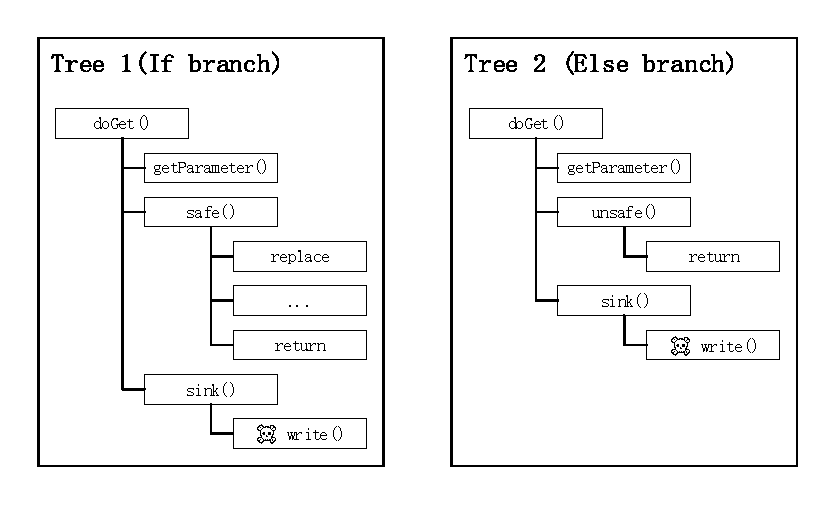
\includegraphics[width=0.9\textwidth]{FIGs/chapter4/taintTree.pdf}
    \caption{\textit{doGet()} 函数的污点传播树}\label{taintTree}
\end{figure}

真实情况下,一个程序中可能存在大量 if-else 语句,可能会导致路径爆炸的问题,因此系统在这里对算法进行了限制,当入口函数的传播树个数大于 300 时,将不再获取子传播树集合,而是直接获取一棵可行的传播树。

得到污点传播树后,对传播树再做一次深度搜索可以将书上的所有节点转化为可以显示在界面上的注解,其算法表示如 算法~\ref{alg:buildAnnotation} 所示。

\begin{algorithm}[!htb]\footnotesize
    \caption{构造污点传播树注解伪代码实现}
    \label{alg:buildAnnotation}
    \KwIn{$n$,污点传播树树根;$depth$,树节点深度,初始化为0;$book$以处理的位置,初始化为$\varnothing$;$annotations$,当前注释集合,初始化为$\varnothing$}
    \KwOut{$R$, 污点传播树的注解集合}
    \SetKwProg{Fn}{Function}{}{}
    \Fn{dfs(n:TreeNode, depth: int, book: Set<SrcAnnotation>, annotations: Set<SrcAnnotation>) : Set<SrcAnnotation> }{
        \If{n is null}{
            \Return{$\varnothing$}
        }
        \If{n in book}{
            \Return{$\varnothing$}
        }
        $R \leftarrow annotations \cup \left\{ getAnnotation(n) \right\} $\\
        $R \leftarrow R \cup dfs(n.firstChild, depth+1, book \cup \{n.location\}, annotations)$\\
        $R \leftarrow R \cup dfs(n.nextSib, depth, book \cup \{n.location\}, A)$\\
        \Return{R}
    }
\end{algorithm}

对于污点传播树的搜索比传播图要简单的多,只要先将当前节点构造成一条注解,再搜索其孩子节点和兄弟节点即可,注意兄弟孩子节点可能为空,因此在搜索前需要判断,若为空值则返回空集,此外,通过算法~\ref{alg:buildTaintTree} 构造的树节点实际上是存在回路的,在打印时需要考虑到这点,因此增加了 book 参数记录,限制当前节点不能循环搜索。在一开始调用时,只需要将 depth 设为 0,book 和 A 设为空集即可。

对于污点传播图的每一个入口函数,可以构造一至多棵污点传播树,对应的就有一至多组注解集合。

\section{程序切片模块的实现}
在设计章节,本文已经对该模块的功能,主要流程和重要类图进行了介绍,在本节中,将从整个流程的控制模块和后向切片两方面介绍该模块的具体实现。\\

\subsection{切片控制模块实现}

\subsubsection{切片控制代码}

切片控制模块的实现代码片段如代码~\ref{code:sliceControl} 所示,该代码出现在 SliceRunner 的 \textit{run()} 方法中,主要功能是调用翻译器和切片器对一个目标项目中的所有漏洞切片,即执行流程图~\ref{sliceProcessing} 上的流程。

代码的第1行首先调用 reportParesr 将项目进行过滤和翻译,得到 taintProject, 接着第 3 行通过项目中的应用 Jar 包和依赖 Jar包,对 slicer 进行配置。接着遍历污点传播类型的漏洞实例,对于每一个实例,获取其污点传播树集合(第11行),接着遍历污点传播树,对每一个污点传播树进行切片(第19行),每完成一个漏洞实例后向监视器汇报进度(第24-25行),并且若是 Joana 类型的切片器,对切片器进行清除缓存的操作,防止缓存过多造成 OOM,最后返回切片项目。\\

\begin{minipage}[!h!t!b!p]{0.9\textwidth}
    \lstinputlisting[language=Java, caption={切片控制模块实现代码片段}, label={code:sliceControl}]{FIGs/chapter4/sliceControl.java}
\end{minipage}

\subsubsection{过滤漏洞实例}

本系统为实现切片预测逻辑和污点传播逻辑的解耦,产生了翻译漏洞报告这一过程。在 Spotbugs 报告类型的翻译器中,主要逻辑在于对漏洞过滤并还原污点传播树。对于污点传播树的还原可以通过对漏洞注解的二次遍历实现,这里不再赘述,本节主要通过代码~\ref{code:sliceFilter},介绍过滤漏洞实例的实现。

\begin{minipage}[!htbp]{0.9\textwidth}
    \lstinputlisting[language=Java, caption={漏洞过滤代码片段}, label={code:sliceFilter}]{FIGs/chapter4/sliceFilter.java}
\end{minipage}

从第 3-4 行可以看出,模块按漏洞类型过滤掉了非污点传播类型漏洞、已经修复的漏洞(在 Spotbugs 中,已经修复的漏洞 \textit{isDead()} 函数返回 True),以及漏洞危害等级为低级的漏洞,在 Spotbugs 中,污点传播类漏洞实例的评级往往是根据污点传播情况制定的,而低级的漏洞往往不存在污点入口点而空有污点汇聚点,这种情况按照当前漏洞观念已经可以判断为误报,不需要本系统处理,在第 6-11 行过滤的漏洞其污点汇聚点没有被其他函数调用(相当于代码~\ref{code:xss} 中的 \textit{sink()} 函数没有被调用),这种漏洞实例也可以直接判断为误报。

\begin{minipage}[!htbp]{0.9\textwidth}
    \lstinputlisting[language=Java, caption={漏洞过滤代码片段}, label={code:caredVulns}]{FIGs/chapter4/caredVulns.java}
\end{minipage}

在按类型过滤漏洞时,使用了白名单过滤方式,目前模块内的白名单如代码~\ref{code:caredVulns}所示,列表中覆盖绝大多数的 Web 安全问题,如XSS、SQL注入和SSRF等。

\subsubsection{分解污点传播树}

在代码~\ref{code:sliceControl} 中,其使用 sliceTaintTree(node) 对一个污点传播树进行切片,该函数具体实现在代码~\ref{code:sliceTree} 中。

% 对污点传播结果的dfs算法 top.anemone.mlsast.core.slice.DFSTaintTree
\begin{minipage}{0.9\textwidth}
    \lstinputlisting[language=Java, caption={漏洞过滤代码片段}, label={code:sliceTree}]{FIGs/chapter4/sliceTree.java}
\end{minipage}
 
 在代码中可以看出,对于待切片的污点传播树,首先将其拆解为污染流集合(第 2 行),再对每一污染流进行切片,将传播树与污染流的映射关系,以及污染流和切片的对应关系放入切片项目中。其中关键点是将污点传播树分解为污染流。
 
 \begin{algorithm}[!htb]\footnotesize
     \caption{从污点传播树中分解污染流集合}
     \label{alg:getTaintFlows}
     \KwIn{$r$: 污点传播树树根}
     \KwOut{$flows$, 污染流的集合}
     $flows \leftarrow \varnothing$\\
     $dfs(r)$\\
     \SetKwProg{Fn}{Function}{}{}
     \Fn{dfs(s: TreeNode): bool}{
        $nextNode \leftarrow s.firstChild$\\
        \While{nextNode != null}{
            \If{nextNode is MethodTreeNode}{
                \If{nextNode.type is Edge.SINK}{
                    $flows \leftarrow flows \cup \{Flow(s.caller, n.location) \}$\\
                    \Return{$true$}\\
                }
                $hasSink \leftarrow hasSink \lor dfs(nextNode)$\\
                \If{hasSink}{
                    $flows \leftarrow flows \cup \{Flow(s.caller, n.location)\}$\\
                    \Return{$hasSink$}\\
                }
            }
            \Else{
                $flows \leftarrow flows \cup \{Flow(s.caller, n.location)\}$\\
                \Return{$hasSink$}\\
            }
            $nextNode \leftarrow nextNode.nextSib$
        }
     }
 \end{algorithm}

算法~\ref{alg:getTaintFlows} 描述了分解过程,算法输入为一个传播树的树根,输出为污染流的集合,首先将初始化一个空的污染流集合,接着通过深度优先搜索得到所有污染流。在搜索过程中,依次遍历当前树节点下的所有孩子节点,如果节点是函数节点,先检查是否是汇聚点函数,如果是则将树根到当前位置作为一个污染流放入集合中,同时返回该函数内有汇聚点,如果不是则递归向下搜索,若该节点的函数内有污点汇聚点,将树根到当前节点位置放入集合中。若节点是返回值节点,则直接将从树根到当前节点的作为污染流放入集合中。

从算法可以看出,污染流实际上是传播树上涉及的每一个函数和其对应的关注点二元组,这里的关注点可能是返回语句,或是调用汇聚点函数的语句,例如,对于图~\ref{taintTree} 中的 Tree 1,可以得到 $doGet() \rightarrow sink()$、$safe() \rightarrow return$和$sink() \rightarrow write()$污染流。\\

\subsection{后向切片的实现}
\subsubsection{基于 Joana 的后向切片}
对于得到的污染流对象,需要由切片器其代码对其后向切片,本系统默认使用Joana对其切片,其主要过程如代码所示,该代码实现于 \textit{JoanaSlicer.computeSlice()} 方法中。

\begin{minipage}[!htbp]{0.9\textwidth}
    \lstinputlisting[language=Java, caption={基于 Joana 的后向切片}, label={code:sliceJoana}]{FIGs/chapter4/sliceJoana.java}
\end{minipage}

代码首先要获取函数 func 的 SDG ,若该函数在缓存中存在,则直接拿出(第 3 行),若不存在,则需要根据配置和入口生成 SDG(第 5$\sim$16 行)。接着使用 SDG 初始化一个 JoanaSDGSlicer,获取关注点行号上的所有 SDGNode 并且对其切片。切片完成后,对其按行号进行排序——这主要保证了每一次对相同污染流的切片的输出一致性。最后将其格式化为字符串。

在 \textit{JoanaSDGSlicer.slice()} 函数主要实现利用 Joana 包中的 SummarySlicerBackward 类对程序进行切片,并对切片的 SDGNode 集合进行过滤。对于需要移除的 SDNode 类型由 isRemovable() 实现,如代码~\ref{code:sliceJoanaRemove} 所示。从代码中可以看到,如果 SDGNode 没有对应源代码、不存在于用户Jar包中、源代码行号小于0、代表异常节点、代表虚节点或抽象节点则将其移除。

\begin{minipage}[!htbp]{0.9\textwidth}
    \lstinputlisting[language=Java, caption={判断 SDGNode 是否需要移除的代码片段}, label={code:sliceJoanaRemove}]{FIGs/chapter4/sliceJoanaRemove.java}
\end{minipage}


\subsubsection{SDG 的生成配置类}
切片需要通过配置生成 SDG,然而默认的 Joana 配置并不具备缺失依赖下生成 SDG 的功能,为此本系统基于最新版本 WALA,重新编译了 Joana,添加自定义配置,缺失依赖的 SDG 生成等功能;当程序规模过大时,生成 SDG 时会消耗过多资源,针对本系统的切片使用场景,本模块切片器实现了限制调用图的切片,这同样是依赖配置实现的,另外,对于异形目录结构的Jar包(如 Spring Web 项目 Jar 包)默认配置会存在找不到类的问题,这依旧依赖配置实现,因此本节将详细介绍这些配置类,这些类的类图如图~\ref{JoanaConfig} 所示。

\begin{figure}[!htb]
    \centering
    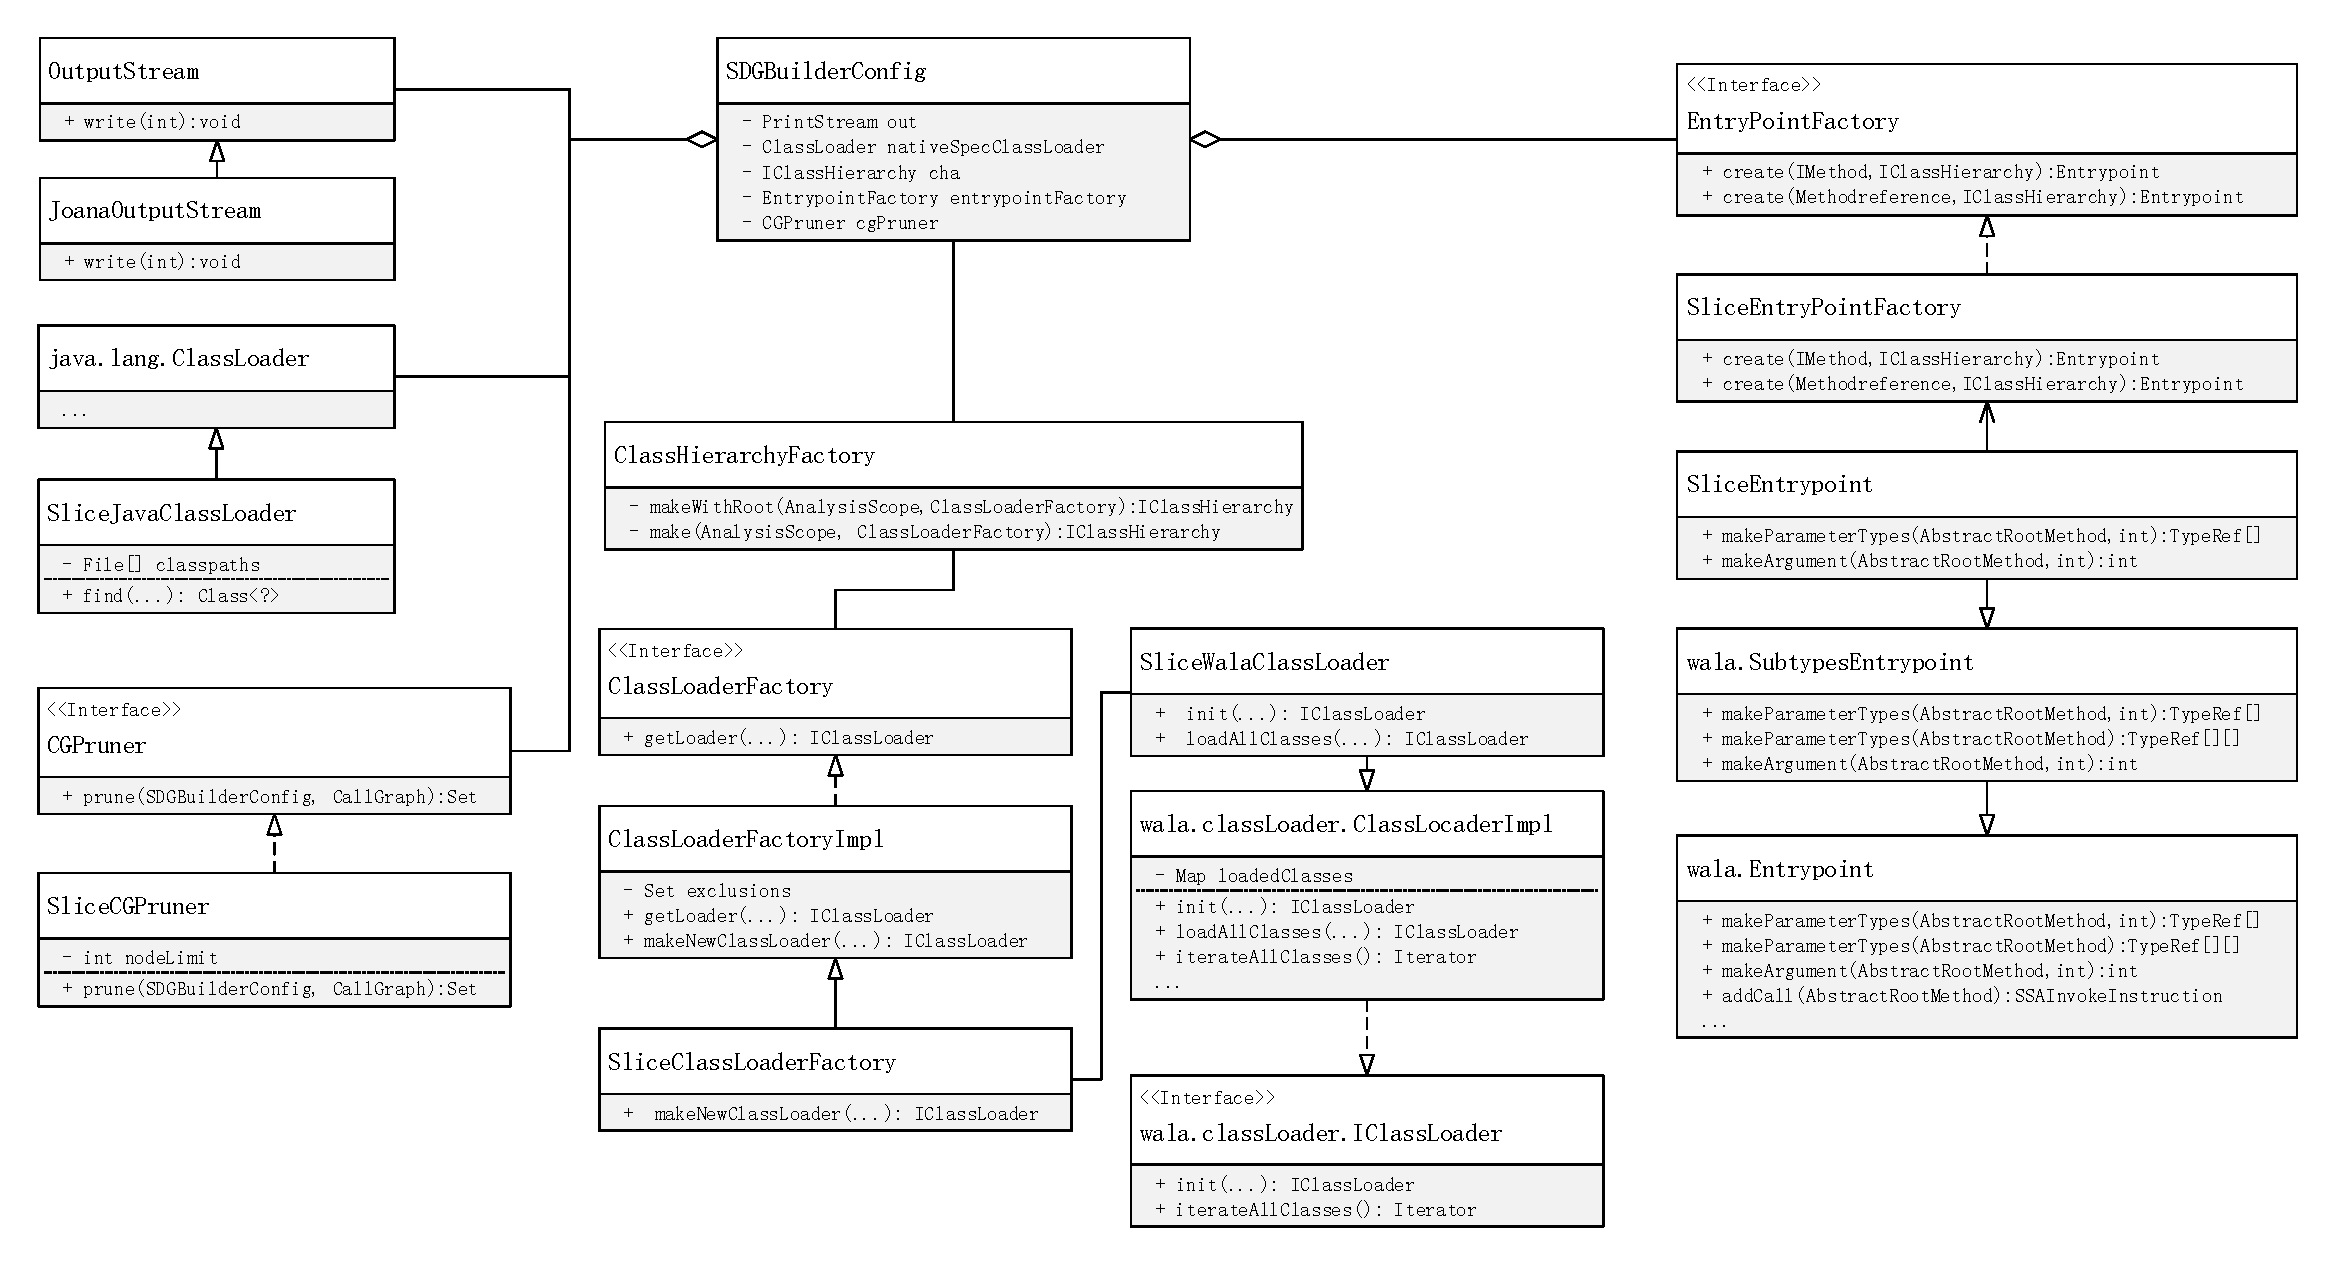
\includegraphics[width=0.9\textwidth]{FIGs/chapter4/sliceConfigClass.pdf}
    \caption{生成 SDG 的配置类图}\label{JoanaConfig}
\end{figure}

为 Joana 打印日志,有 JoanaOutputStream 类,其继承 Java 原生的 OutputStream, \textit{write()} 函数用来向控制台打印日志信息,其实例保存于配置的 out 属性中。

SliceJavaClassLoader、SliceClassLoaderFactory 和 SliceWalaClassLoader 用于解决异形 Jar 包找不到类的问题,例如,Springboot 的项目 Jar 包中,类文件的地址前缀为 “$BOOT-INF/classes/\langle package \rangle.\langle class \rangle.class $”,对于 Joana 切片来说,其首先通过 ClassHierarchyFactory 工厂类获取类层次图(IClassHierarchy),类层次图中包含了切片器能够分析的所有类,构造类的层次图首先会扫描 Jar 包中的所有 .class 文件作为类文件,并将其目录作为包名和类名,如:从“a/b/XSS.class”得到类“a.b.XSS”,工厂类中函数 \textit{makeWithRoot()} 和 \textit{make()} 都是构建调用图的函数,区别在于 \textit{makeWithRoot()} 支持缺失依赖的层次图生成,这将在后文详细介绍,它们的第一个参数是分析范围,该对象可以通过传入的 Jar 包路径创建,而第二个参数为 Jar 包的类加载器工厂类(ClassLoaderFactory),注意这里的类加载器不等同于 Java 原生的 Classloader。类加载器 IClassLoader 为一接口,其中定义了 \textit{iterateAllClasses()} 方法用于遍历分析范围类的所有类,首先为了解决类查找问题,需要在遍历时获取这些 Jar 包的正确类名,即重写 ClassLoader 并建立对应的工厂类。Joana 默认的(准确的说是 Joana 借助 WALA 的)类加载器为 ClassLoaderImpl,其 \textit{init()} 方法通过 \textit{loadAllClasses()} 将 Jar 中的所有类读取至缓存,当调用 \textit{iterateAllClasses()} 时,只需遍历缓存中的类即可,因此本模块的 SliceWalaClassLoader 继承了 ClassLoaderImpl 并重写了 \textit{loadAllClasses()} 方法,其实现如代码~\ref{code:sliceWalaClassLoader} 所示,可以看到代码第 9-10 行,当包名中存在“/classes/”目录时,去除“/classes/”及前部分字符,只留下包名和类名。

接着模块需要解决类实际加载的问题,模块通过自定义 Java 原生 ClassLoader(SliceJavaClassLoader)解决该问题,该类实现代码如代码~\ref{code:sliceJavaClassLoader} 所示,其关键在于代码第 9 行,即通过字符串尾部匹配来判断 classpath 下是否包含文件,如果包含则读取该类的内容至比特数组 classByte 中。 

最后,将 ClassHierarchyFactory 产生的类层次图配置在 SDGBuilderConfig 实例的 cha 属性中。

\begin{minipage}[!htbp]{0.9\textwidth}
    \lstinputlisting[language=Java, caption={SliceWalaClassLoader 代码实现}, label={code:sliceWalaClassLoader}]{FIGs/chapter4/sliceWalaClassLoader.java}
\end{minipage}

\begin{minipage}[!htbp]{0.9\textwidth}
    \lstinputlisting[language=Java, caption={自定义JavaClassLoader}, label={code:sliceJavaClassLoader}]{FIGs/chapter4/sliceJavaClassLoader.java}
\end{minipage}


很多用户提交的Jar包并不包含第三方包依赖信息,默认 Joana 无法完成切片,其关键问题在于以下两点:(1)当类继承于其他第三方包中类时,Joana 由于无法找到第三方类而无法构造该类;(2)当函数参数类型为第三方包中类时,Joana 由于无法找到类原型无法分析。

对于第一点,模块重新编译了 Joana 使其依赖于高版本的 WALA,在生成类层次图是,使用 \textit{makeWithRoot()} 方法生成,该方法在生成类层次结构图时,若该类的父类为搜索范围之外的类,则将其继承自 Object 类(在 Java 中 Object 类是所有类的父类)。

对于第二点,为此模块在 SliceEntrypoint 类中重新写了 Entrypoint 类的\textit{ makeParameterTypes()} 和 \textit{makeArgument()} 方法,\textit{ makeParameterTypes()} 用在函数调用语句发生时,返回函数调用参数类型,这里当调用的参数类型为范围外的类时,函数返回一个伪造的类型,\textit{ makeArgument()} 用于当函数调用发生时,为实参创建一个实例,并返回实例节点的序号,这里当实参类型为范围外的类时,伪造一个虚节点加入序号表中,并将其返回。
此外,模块实现 SliceEntrypoint 类的工厂类 SliceEntryPointFactory,并将其配置在 SDGBuilderConfig 实例的 entrypointFactory 属性中。

\begin{minipage}[htbp]{0.9\textwidth}
    \lstinputlisting[language=Java, caption={NodeLimitPruner 的实现}, label={code:slicePruner}]{FIGs/chapter4/slicePruner.java}
\end{minipage}


用户上传的实际程序规模不可控,对其进行完整切片很可能造成物理资源耗尽或是程序崩溃,为此,模块在 \textit{NodeLimitPruner.prune()} 中实现了对调用图剪枝来限制切片规模,代码~\ref{code:slicePruner} 描述了其过程。首先,初始化需要保留的CGNode集合 keep,向搜索队列中加入抽象函数节点和真实函数节点,向搜索队列中加入真实入口函数节点,接着通过广度优先搜索,向 keep 中加入不超过 nodeLimit 数量的节点,最后返回 keep 即可。


下面以代码~\ref{code:xss}中 \textit{doGet()} 函数为例,说明剪枝过程,首先,WALA 会计算出如图~\ref{prune} 所示的函数调用图,\textit{fakeRootMethod()} 是 WALA 的一个抽象函数,它是所有调用图的入口,遍历时通过该函数寻找其他函数,接着该函数会连向 \textit{fakeWorldClinit()}——该函数也是 WALA 的抽象函数,WALA 通过该函数调用其他类的构造方法;该函数还会连向\textit{XSS.<init>()} ,它是 XSS 类的构造方法,最后函数连向真正需要进行切片的入口方法 \textit{doGet()},在 \textit{doGet()} 中由于调用其他函数,又会出现其他方法节点。在剪枝时,首先需要将\textit{fakeRootMethod()} 方法加入 keep,否则无法进行遍历找到其他方法;接着加入入口方法 \textit{doGet()} ,随后按顺序依次加入 \textit{safe()} 和 \textit{unsafe()}方法,如果限制调用节点数为 4,那么 \textit{sink()} 节点将被剪枝,即最后保留的函数依次为 \textit{fakeRootMethod()}、 \textit{doGet()}、\textit{safe()} 和 \textit{unsafe()},可以看到在搜索时,代码还忽略了非应用定义的方法,如\textit{getParameter()}、\textit{startsWith()} 等,这是为了在有限集合内尽可能多的保留程序特性,而省略其共性(因为不管是安全和非安全代码,这些非应用函数内切片内容不变),同时被删去的\textit{sink()} 函数也并不是被彻底忽略,因为它会在其他子污染流中被计算。
    
\begin{figure}[!htb]
    \centering
    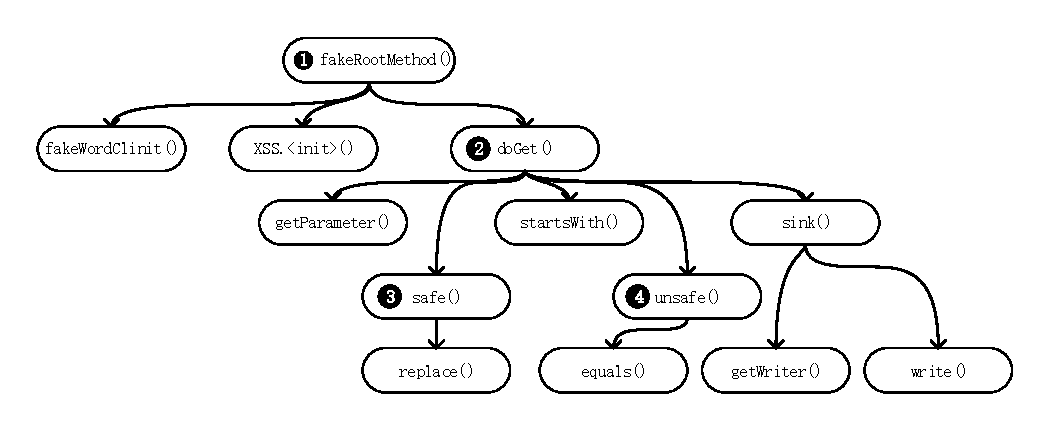
\includegraphics[width=0.9\textwidth]{FIGs/chapter4/prune.pdf}
    \caption{限制调用图示意图}\label{prune}
\end{figure}


\section{数据处理模块的实现}

数据处理模块将程序切片进行泛化和向量化处理,以保证神经网络的泛化性能,本节就泛化处理和向量化两方面说明该模块的实现。\\

\subsection{泛化处理}

在设计阶段,本文已经介绍了模块对程序切片的泛化主要分泛化数字常量、泛化字符串常量、泛化变量、泛化函数调用和泛化包名方法名五个方面,下面以 $unsafe() \rightarrow return(line:31)$ 函数的代码切片~\ref{code:sliceDemo}为例,介绍这些泛化的具体含义。

\begin{minipage}[!htbp]{0.9\textwidth}
    \lstinputlisting[language=Java, caption={\textit{unsafe()} 函数的代码切片}, label={code:sliceDemo}]{FIGs/chapter4/sliceDemo.txt}
\end{minipage}

首先是泛化数字常量,数字常量在切片中往往带有数据信息,然而程序切片中的数字返回往往变化很大,为了泛化总结出共性,模块将三位数及以上的整数同一替换为“N3P”,将三位数及以上的负整数替换为“NN3P”,将科学计数法的数字替换为“NSMALL”,剩余三位数及一下数字将其“\#()”去除保留数字字符串,因为系统认为这些数字的具体值有更为重要的信息,如在示例切片第 3 行中的“\#(0)”,将其替换为 “0”。

字符串常量在切片代码中非常常见,其内容也可能是判断一个切片是否是安全的重要标准,如 SSRF 漏洞切片中发现有 “http://site”开头的字符串,那么漏洞很可能是误报,或是注入型漏洞出现特殊符号的替换字符串,那么这些漏洞也很可能是误报。因此,对于字符串要做特殊泛化处理,首先,若包含如“HTTP”,“HTTPS”且长度大于其4的字符串,将其泛化为“URL”;此外,若字符串长度大于 2,因为这些字符串是清洁字符串的概率较小,将其泛化为 “STR S\{i\}”的形式,i 指该字符串为切片中出现的第 i 个字符串;否则保留其本身,因为其本身很可能是清洁类字符串。例如在第 2 行切片中出现的“\#(clean)”,则将其泛化为 “STR S1”(其为切片中出现的第一字符串)。

由于切片对象为静态单赋值形式(SSA),以“v\{数字\}”表示的变量在切片中很常见,但是由于切片原因,这些数字并不是自然增长的,因此在泛化流程中,对其出现顺序进行映射,将其泛化为“VAR V\{i\}”的形式,其中 i 代表该变量是第 i 个出现在切片中的,例如第 2 行、第 3 行和第 4 行出现的 v6 变量,将其泛化为“VAR V1”,即该变量第 1 个出现在切片中。

函数调用的泛化主要是针对于调用切片和返回,对于调用切片,如第 2 行,将其调用函数前的“.”去除,若有形参(“\$”开头的变量)也将其去除,因为形参名称与漏洞本身无关,并在括号前后加空格,当做完经过该步骤后,第 2 行切片的函数调用部分泛化为“VAR V1 = p1 equals ( STR S1 ) ”,若函数调用返回为对象,则将其下划线形式改为“.”连接的形式,如最后一行中的“Ljava/lang/String”变为“java.lang.String”。

泛化包名方法名,此类泛化主要对于 ENTER 类型的节点,如第 1 行,这里需要将切片拆分为“包名\_方法名\_函数参数类型”,如将“demo.XSS.unsafe(java.la-\\ng.String)”泛化为“demo XSS unsafe ( java.lang.String )”。\\

数字常量、字符串常量和变量的泛化分别在 Preprocessing 类中 \textit{processNumber()}、\textit{processStr()} 和 \textit{processVer()} 中实现,对于函数调用和包名方法名的泛化在 \textit{processType()} 实现

\subsection{建立单词表与向量化}

在本模块 Tokenizer 类中,泛化后字符串首先生成单词表,再按照单词表可以对句子进行向量化。其实现代码如代码~\ref{code:preTokenize} 所示。

\begin{minipage}[!htbp]{0.9\textwidth}
    \lstinputlisting[language=Python, caption={建立单词表和向量化的实现}, label={code:preTokenize}]{FIGs/chapter4/preTokenize.py}
\end{minipage}

\textit{build\_dict()} 方法输入为切片数据集,方法首先建立一个空的字典 \_dict 和词频表 word\_freq,接着遍历数据集中的所有切片,按空格拆分,并开始统计词频,遍历结束后,根据词频表,将词频大于 freq\_gt 的单词放入单词表,单词进入单词表的顺序将成为其id,小于等于该词频的单词会被映射为“UNK”,方法最终返回一个单词字典。
\textit{encode()} 方法用于将一个切片数据向量化,其只需要将泛化后的单词序列分解为单词,再通过字典将每一个单词映射为 id 即可,方法最终返回为一个句子的向量。\\

\section{误报预测模块的实现}

\subsection{误报预测控制}
误报预测控制负责执行图~\ref{predictProcessing} 中的主要流程,其代码如~\ref{code:predictRunner} 所示。

\begin{minipage}[!htbp]{0.9\textwidth}
    \lstinputlisting[language=Java, caption={误报预测控制逻辑的实现}, label={code:predictRunner}]{FIGs/chapter4/predictRunner.java}
\end{minipage}

代码遍历 sliceProject 中的每一个实例、每个实例中的每个污点传播树以及每个传播树中的污染流,从代码 20$\sim$23 行可以看出,只要树中有一条污染流是安全的,那么整个传播树就是安全的,因为污点无法向下传播至汇聚点,对应的安全流会保存到 safeFlows 集合中。从第 27 行可以看到,只有当所有的污点传播树都是安全时,一个漏洞实例才可判断为误报,最后,将是否为误报的结果和安全的流放入预测项目中作为证明放入项目中。\textit{flowIsSafe()} 在调用远程预测服务前,会先检查缓存是否已有记录,若存在记录则直接将其返回,否则调用远程服务。\\

\subsection{误报预测时序图}
误报预测模块存在客户端至服务器调用流程,本文通过时序图~\ref{predictTime} 说明误报预测的调用实现。

\begin{figure}[!htb]
    \centering
    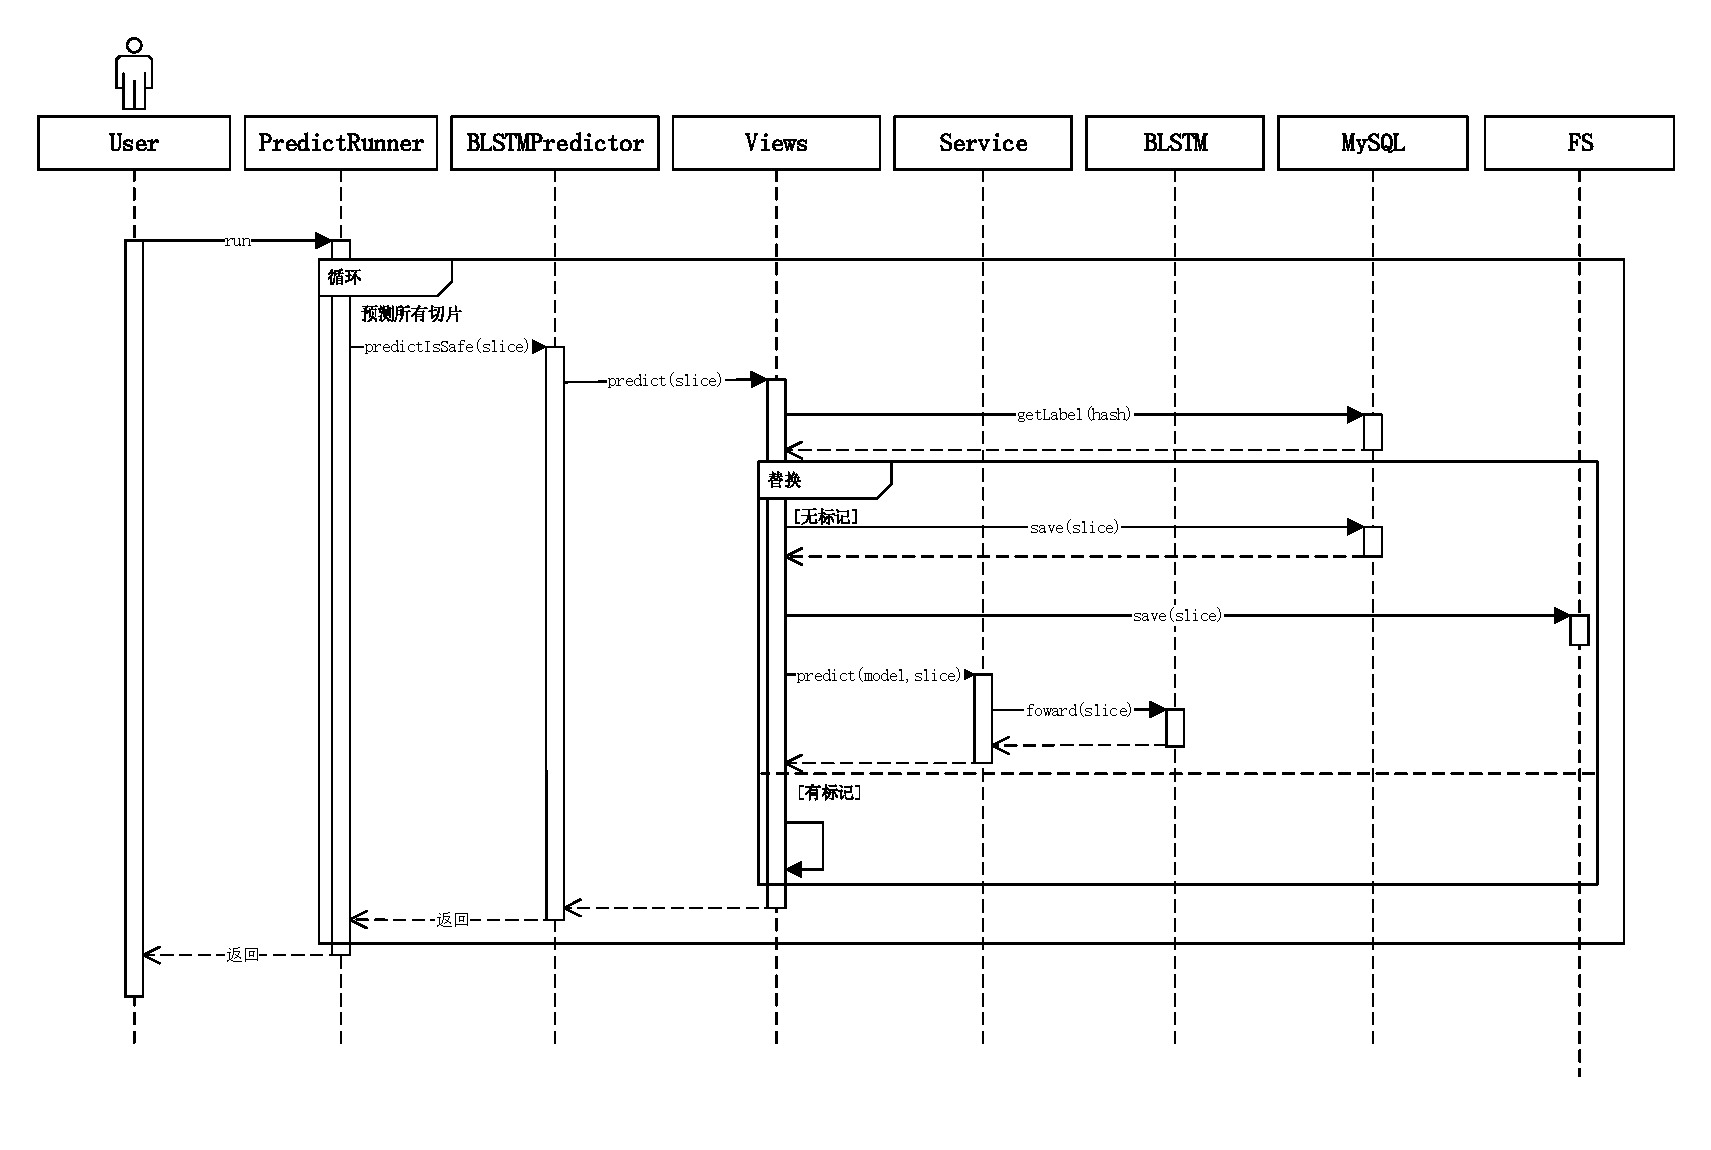
\includegraphics[width=0.9\textwidth]{FIGs/chapter4/predictTime.pdf}
    \caption{误报预测时序图}\label{predictTime}
\end{figure}

用户首先发起对污点传播报告的预测请求,接着预测控制逻辑进入循环,对于每一个切片调用 BLSTMPredictor 进行预测,BLSTMPredict 为远程服务的本地代理,其会向远程服务器发送预测请求,服务器视图层收到预测请求后,首先从数据库查找该切片是否有标记,如果有标记则优先返回标记数据,否则先将切片依次保存至数据库和本地文件系统中,再向预测服务发起预测请求,预测服务收到请求后发送给 BLSTM 模型,模型将预测结果依次返回至用户。\\

\subsection{漏洞标记时序图}

本模块的另一重要流程在于对漏洞实例的标记,时序图~\ref{labelTime} 展示了漏洞标记的实现过程。

用户可以对一个漏洞进行误报或正报的标记,首先看误报标记流程,对于一个误报漏洞实例,用户需要提供误报原因,即指定污点消失于那些污染流中,接着GUI界面会生成一个 Label 实例并向预测器发送标记为安全污染流的请求,本地预测器会将请求转发到服务端的 View 层,View 层收到请求后将标记数据依次写入数据库和本地文件中,由于污染流哈希的唯一性,当数据库存在已有标签时会自动覆盖。

对于一个正报标记,用户需指定漏洞实例的一个可利用的传播树,因为一个真实的漏洞的只要有一棵传播树的污点传播成立,该漏洞就真实存在,GUI 收到请求后会遍历传播树相关的所有切片,并发送标记为不安全的标签。对于每一个不安全标签的标记时序与安全标记时序相同,这里不再赘述。


\begin{figure}[htbp]
    \centering
    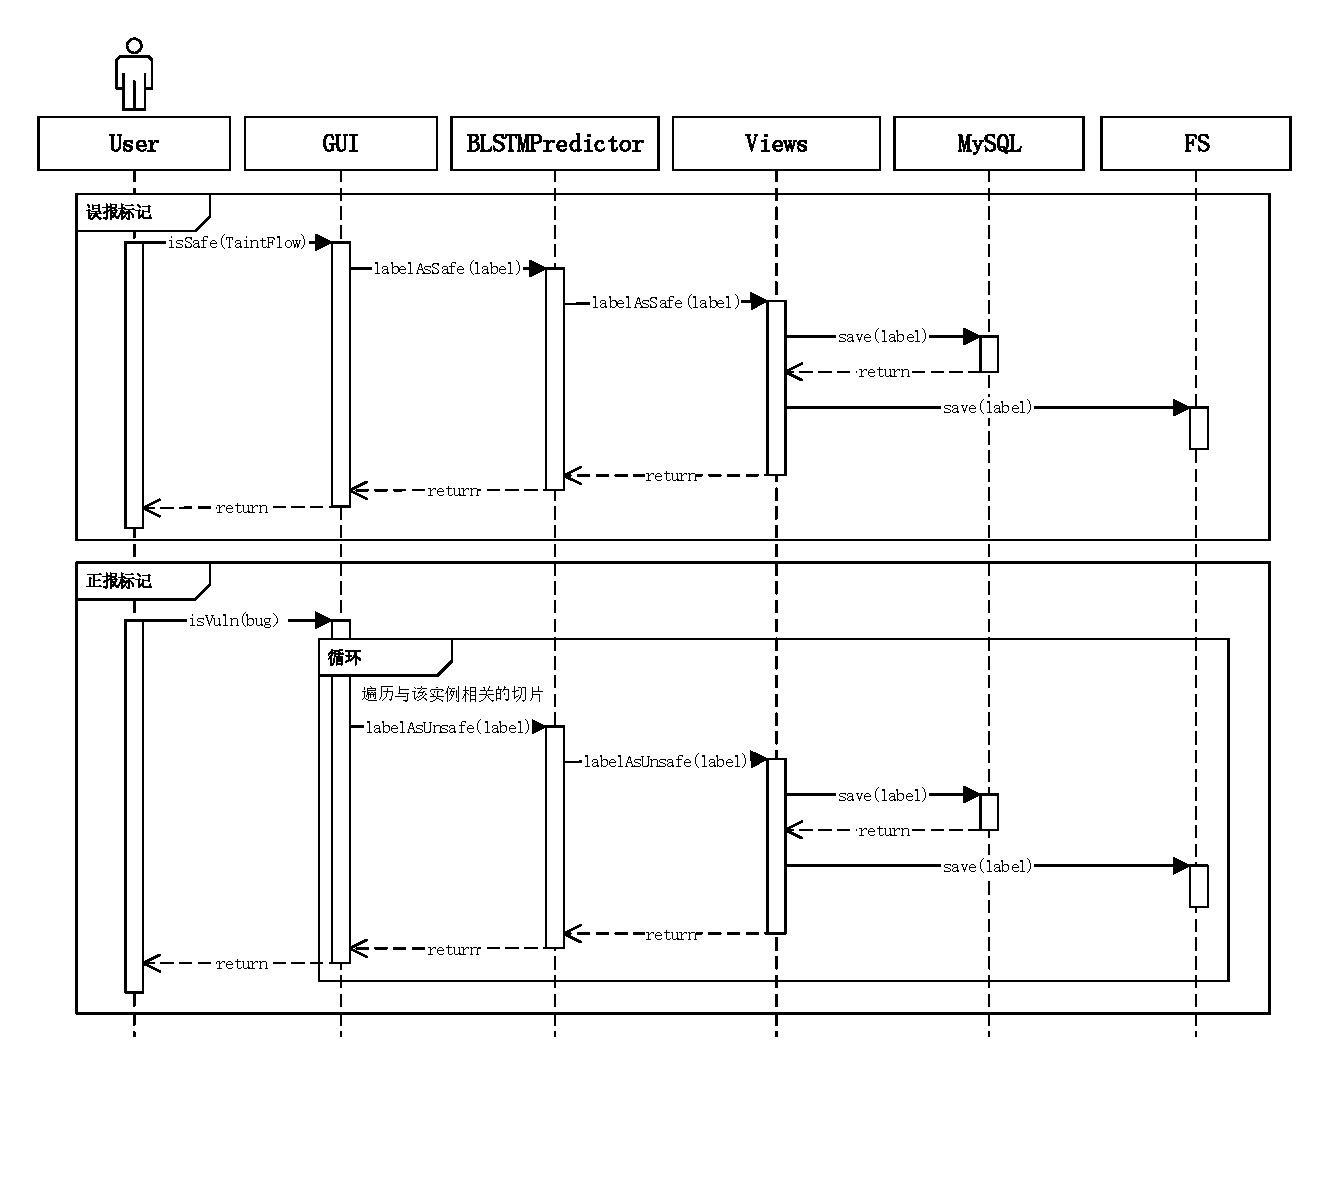
\includegraphics[width=0.9\textwidth]{FIGs/chapter4/labelTime.pdf}
    \caption{漏洞标记时序图}\label{labelTime}
\end{figure}

\subsection{批训练过程}

用户在 Web 端可以发起训练任务,Celery Worker 收到训练任务后,会调用训练服务按指定配置训练 BLSTM 神经网络。

% https://www.zhihu.com/question/32673260
该模型训练时的输入为切片向量集合,对应标记集合,输出为一个训练好参数的 BLSTM 模型。由于程序切片大小有差异,切片向量长度也是不一致的,对于时序型神经网络 BLSTM 来说,本身就具有接受不定长向量的能力,然而在实际训练时,为了保证训练效率和效果,往往会将一批切片向量和对应标记合并为一批数据输入神经网络,再进行权重更新——批训练~\cite{imageNet,trainLonger,largeBatchLSTM},这时一组切片向量需要转换为二维向量,即需要对末尾补 0,因此在BLSTM模型中,要考虑无效数据。

Pytorch 的 DataLoader 对象可手动指定校对函数 \textit{collate\_fn()},该函数用于从数据集加载数据后,对数据进行最后处理,本模块根据需要构造的校对函数如代码~\ref{code:collateFn} 所示。

\begin{minipage}[!htbp]{0.9\textwidth}
    \lstinputlisting[language=Python, caption={DataLoader 的加载器}, label={code:collateFn}]{FIGs/chapter4/collateFn.py}
\end{minipage}

可以看出,该函数的输入为一个向量化类和一批数据集合,该集合中存放切片字符串和对应标记对,对于每一个标记对,首先调用预处理模块对其泛化和向量化(第 3 行),接着按切片长度从长到短对一批数据排序,获取每条切片的长度记为 data\_length 变量,使用 Pytorch 预定义的函数 \textit{rnn\_utils.pad\_sequence()} 对已排好序的一批数据进行补 0,此时 data\_x 类型已由原先的 list 类型变为二维张量(Tensor)类型,最后将这批数据的标记作为一维向量,最后函数返回切片张量(二维),切片长度向量(一维)和标记向量(一维)。

接着切片张量和切片长度向量将传递至 BLSTM 类的 forward() 方法中,代码~\ref{code:blstm} 展示了神经网络后向传播的细节。

\begin{minipage}[!htbp]{0.9\textwidth}
    \lstinputlisting[language=Python, caption={DataLoader 的加载器}, label={code:blstm}]{FIGs/chapter4/blstm.py}
\end{minipage}

首先,对于切片张量进行词嵌入,即使用向量替换每一个词,其输出的 embeds 为三维张量,注意这里词嵌入已经指定了 padding 值,即将补齐用的数字映射为全 0 向量。接着使用 Pytorch 定义的 \textit{rnn\_utils.pack\_padded\_sequence()} 函数将实际上不等长的切片向量打包,打包数据传递至 BLSTM 层, BLSTM 层输出还原至三维张量,注意,此时张量规模为记录数 $\times$ 最长语句长度 $\times$ BLSTM神经元个数。 \textit{get\_last\_output()} 会获取该三维张量上每一记录的双向传播时最后一时刻的神经元输出,并整合为一二维张量,最终输出到线性层,线性层返回预测结果。

\begin{figure}[!htb]
    \centering
    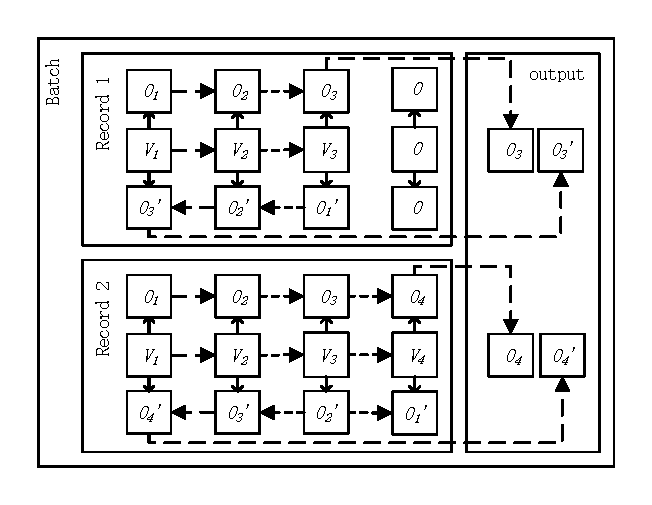
\includegraphics[width=0.9\textwidth]{FIGs/chapter4/blstmFoward.pdf}
    \caption{批处理训练示意图}\label{blstmForward}
\end{figure}

图~\ref{blstmForward} 展示了批处理训练的具体做法,假设一批数据中存在两条数据 record 1 和 record 2, 它们有效的切片向量长度为 3 和 4,将它们的单词做词嵌入后,得到张量$\{V_{1},V_{2},V_{3}\}$ 和$\{V_{1},V_{2},V_{3},V_{4}\}$,经过 BLSTM 神经网络后,正反方向分别产生了每个时刻上的输出,此时对于记录 1 来说,需要提取最后一个时刻的神经元输出,即 $O_3$ 向量和 $O_3'$ 向量,并将其合并,对于记录 2 来说,提取并合并为 $\left[O_{4}, O_{4}'\right]$,该二维张量输入至线性层,得到最终分类结果。也就是说,线性层神经元个数为 BLSTM 神经元个数的两倍。

\section{系统测试与运行展示}
\subsection{测试目标}
本系统测试主要有功能测试、健壮性和性能测试,在功能测试方面主要对系统功能的正确性进行测试;而健壮性和性能测试主要关注于本系统在扫描各类被测应用时的程序不崩溃,并能在合理时间内返回数据。

在功能测试中,主要对第~\ref{sec:demand} 节提出的需求和用例进行测试,对污点分析、程序切片、预处理和误报预测各个模块的生成测试用例并对其进行测试。在健壮性测试中,主要对系统输入各类 Jar 包,检查系统是否能否在规定时间内产生扫描报告。

表~\ref{tab:testenv}为测试的软硬件环境,在硬件方面,由于扫描任务是计算密集型任务,所以客户端选择了 CPU 较高配置的 E5-2630 和内存为 32G,并将 JVM 参数调整为“-Xmx8g -Xss500m”,服务端的硬件配置与客户端相同,软件上有 Pytorch、Django、Celery、MySQL、Redis 等。

\begin{table}[!htbp]\footnotesize
    \centering
    \caption{系统测试软硬件环境}
    \begin{tabular}{cll}
        \toprule
        \multicolumn{2}{c}{设备与软件} & 备注信息 \\
        \midrule
        \multirow{3}[2]{*}{客户端} & CPU   & 型号为 Intel(R) Xeon(R) CPU E5-2630 v3 @ 2.40GHz \\
        & 内存    & 大小为 32G \\
        & Java  & JVM 参数为“-Xmx8g -Xss500m ”\\
        \midrule
        \multirow{7}[2]{*}{服务端} 
        & CPU   & 型号为 Intel(R) Xeon(R) CPU E5-2630 v3 @ 2.40GHz \\
        & 内存    & 大小为 32G \\
        & Pytorch & 版本为 1.3.1 \\
        & Django & 版本为 2.2.5 \\
        & Celery & 版本为 4.4.0 \\
        & MySQL & 版本为 8.0.12 \\
        & Redis & 版本为 3.0 \\
        \bottomrule
    \end{tabular}%
    \label{tab:testenv}%
\end{table}%

\subsection{功能测试}
本章节主要针对各个模块的主要功能设计测试套件,并对每个测试套件进行具体测试。测试套件如表~\ref{testsuitcase} 所示。

\begin{table}[!htb]\footnotesize %label table
    \centering
    \caption{系统测试用例套件}
    % l - left, r - right, c - center. | means one vertical line 这里声明的是表格单元中的内容如何对齐
    \begin{tabular}{L{0.5cm}L{2cm}L{3cm}L{7cm}}
        \toprule
        \textbf{ID} & \textbf{所在模块} &\textbf{测试功能} &\textbf{测试内容}\\
        \midrule
        TS1 & 污点分析模块 & 基于污点分析的静态扫描  & 提交扫描任务,系统能够将污点分析结果显示在用户界面。\\
        TS2 & 污点分析模块  & 污点分析结果的存取 & 对于一个污点分析结果,系统可以将其保存,并在打开时导入。\\
        TS3 & 程序切片模块  & 程序切片 & 对于一个污点分析项目,对每一个漏洞进行切片,生成程序切片项目\\
        TS4 & 预处理模块   & 切片泛化与向量化 & 对于一个切片文本,对其进行泛化和向量化\\
        TS5 & 误报预测模块  & 预测漏洞安全性 & 对于一个漏洞实例,利用模型预测其是否为误报\\
        TS6 & 误报预测模块  & 标记漏洞安全性 & 对于一个漏洞实例,标记该漏洞是否为误报\\
        TS7 & 误报预测模块  & 模型训练 & 指定模型训练配置,根据配置训练模型\\
        \bottomrule
    \end{tabular}
    \label{testsuitcase}
\end{table}

在污点分析模块,主要有测试套件 TS1,对用户提交的 Jar 包集合进行污点分析,并将污点分析结果以漏洞实例和对应若干棵污点传播树的形式返回给用户;测试套件 TS2,用户对于污点分析结果,进行存取操作。其包含的测试用例如表~\ref{testcase:taint} 所示,TS1 中含一个测试用例 TC1-1;TS2 套件中含两个测试用例,TC2-1 和 TC2-2, 分别测试对于结果的保存和读取。经过测试,得出的测试结果与预期结果相符,测试用例全部通过。

\begin{table}[!htbp]\footnotesize
    \centering
    \caption{基于污点分析的静态扫描测试用例}
    % l - left, r - right, c - center. | means one vertical line 这里声明的是表格单元中的内容如何对齐
    \begin{tabular}{L{0.07\textwidth}L{0.2\textwidth}L{0.18\textwidth}L{0.3\textwidth}L{0.09\textwidth}} 
        \toprule
        \textbf{ID}&\textbf{说明} & \textbf{输入}&\textbf{预期输出}&\textbf{测试结果}\\
        \midrule
        TC1-1 & 污点分析 & 用户提交的 Jar 包  & 污点分析结果(显示到界面) & 通过 \\
        TC2-1 & 污点分析结果保存 & 污点分析结果  & 记录分析结果的XML文件 & 通过 \\
        TC2-2 & 污点分析结果读取 & 记录分析结果的XML文件  &  污点分析结果 & 通过 \\
        \bottomrule
    \end{tabular}
    \label{testcase:taint}
\end{table}

在程序切片模块,主要有一个测试套件TS3,即测试系统能否成功将污点分析项目转化为切片项目,在切片项目中,存在污点传播树和其对应的污染流,每个污点传播对应一条切片。该测试套件对应的测试用例如表~\ref{testcase:slice} 所示,其主要包含有 TC3-1,对上一模块产生的分析结果进行处理,从报告中还原污点传播树;TC3-2,拆解污点污点传播树,将传播树拆解为子污染流的集合;TC3-3,对一个污染流进行后向切片,由于 Joana 自身存在一定不稳定,当切片成功时,程序返回切片文本,在切片失败时扫描任务不崩溃,并返回错误原因。经过测试,以上测试用例输出均与预期相符,测试全部通过。

\begin{table}[!htb]\footnotesize
    \centering
    \caption{程序切片测试用例}
    % l - left, r - right, c - center. | means one vertical line 这里声明的是表格单元中的内容如何对齐
    \begin{tabular}{L{0.07\textwidth}L{0.2\textwidth}L{0.18\textwidth}L{0.3\textwidth}L{0.09\textwidth}}
        \toprule
        \textbf{ID}&\textbf{说明} & \textbf{输入}&\textbf{预期输出}&\textbf{测试结果}\\
        \midrule
        TC3-1 & 处理污点分析结果  & 污点分析结果 & 漏洞实例及其对应传播树集合 & 通过\\
        TC3-2 & 拆解污点传播树  & 污点传播树 & 子污染流集合 & 通过\\
        TC3-3 & 污染流后向切片  & 污染流 & 切片文本(若失败返回错误原因) & 通过\\
        \bottomrule
    \end{tabular}
    \label{testcase:slice}
\end{table}

数据预处理模块的测试套件为 TS4,其用于测试模快是否能对于一个切片文本进行正确泛化和向量化处理。其包含的测试用例如表~\ref{testcase:preprocessing} 所示,TC4-1 用于测试预处理模块能否对于一个切片文本进行有效泛化处理,对其输出单词序列;TC4-2 用于测试模块对于单词序列集合,能否将其转化为向 量集合和对应的单词表,在输入时,单词表为可选项,若不存在单词表则新建,存在则根据已有单词表进行向量生成。经过测试,以上测试用例输出均与预期相符,测试全部通过。

\begin{table}[!htb]\footnotesize
    \centering
    \caption{数据预处理模块测试用例}
    % l - left, r - right, c - center. | means one vertical line 这里声明的是表格单元中的内容如何对齐
    \begin{tabular}{L{0.07\textwidth}L{0.2\textwidth}L{0.18\textwidth}L{0.3\textwidth}L{0.09\textwidth}}
        \toprule
        \textbf{ID}&\textbf{说明} & \textbf{输入}&\textbf{预期输出}&\textbf{测试结果}\\
        \midrule
        TC4-1 & 泛化处理  & 切片文本 & 单词序列 & 通过\\
        TC4-2 & 向量化处理  & 单词序列集合和单词表(可选) & 单词对照表和向量集合 & 通过\\
        \bottomrule
    \end{tabular}
    \label{testcase:preprocessing}
\end{table}

误报预测模块的测试套件为 TS5;TS6,对漏洞实例安全性进行标记;TS7,对已有新数据进行模型训练。它们对应的测试用例如表~\ref{testcase:predict} 所示,安全性实例预测套件对应的测试用例有 TC5-1,对切片文本进行安全性预测,由于切片文本与污染流成一一对应关系,切片文本安全即污染流安全,测试检查系统是否能返回预测结果,并同时将污染流保存到文件系统和数据库中;TC5-2,对一个漏洞实例进行误报预测,测试给定任意漏洞实例和对应传播树的集合,系统能否返回漏洞是否为误报。

安全性标记对应的测试套件为 TS6,测试用例有 TC6-1,标记污染流安全性,对于单个污染流标记其是否安全,系统需要将该标记数据存储至数据库和文件系统中,更新预测结果;TC6-2,标记可利用的传播树,系统需要将其对应的所有污染流标记为不安全,当漏洞的所有污染传播树无法传播污点时,对漏洞也应标记为不安全。

模型训练的测试套件为 TS7,对应的测试用例有 TC7-1,用户在后台新建训练配置,系统将其配置保存至数据库;TC7-2,用户发起训练请求,系统异步完成请求,并将训练好的模型保存至数据库和文件系统。经过测试,以上测试用例输出均与预期相符,测试全部通过。 

\begin{table}[!htb]\footnotesize
    \centering
    \caption{误报预测模块测试用例}
    % l - left, r - right, c - center. | means one vertical line 这里声明的是表格单元中的内容如何对齐
    \begin{tabular}{L{0.07\textwidth}L{0.2\textwidth}L{0.18\textwidth}L{0.3\textwidth}L{0.09\textwidth}}
        \toprule
        \textbf{ID}&\textbf{说明} & \textbf{输入}&\textbf{预期输出}&\textbf{测试结果}\\
        \midrule
        TC5-1 & 切片文本安全性预测 & 污染流和对应切片 & 预测结果,同时污染流保存到文件系统和数据库 & 通过\\
        TC5-2 & 漏洞误报预测  & 漏洞实例和对应传播树集合 & 漏洞是否为误报 & 通过\\
        TC6-1 & 标记污染流  & 污染流切片和标记 & 更新预测结果,标记存储至数据库和文件系统中 & 通过\\
        TC6-2 & 标记可利用的传播树  & 污点传播树 & 更新预测结果,所有对应的污染流标记为不安全并存储至数据库和文件系统 & 通过\\
        TC7-1 & 新建训练配置 & 训练配置 & 生成配置存储至数据库 & 通过\\
        TC7-2 & 发布训练任务 & 训练任务请求 & 异步进行任务训练,并将训练完成的数据保存到数据库和文件系统 & 通过\\
        \bottomrule
    \end{tabular}
    \label{testcase:predict}
\end{table}

\subsection{健壮性和性能测试}

为了测试本系统的健壮性和性能,本文选择 Maven 中央仓库流行度 Top 100 的项目,在每个项目选择使用最多的构建版本作为测试对象~\footnote{\url{https://mvnrepository.com/popular?p=1},抓取时间为 2019年10月24日,当前流行度榜单可能已经发生变化} 批量建立扫描任务进行测试,对于一个项目,本文将系统的最大扫描时间设为 4 小时,如果超过该时间系统仍未返回结果,则认为系统扫描失败,表~\ref{robustTest} 列出了测试结果。

\begin{table}[!htb]\footnotesize
    \centering
    \caption{健壮性和性能测试结果}
    % l - left, r - right, c - center. | means one vertical line 这里声明的是表格单元中的内容如何对齐
    \begin{tabular}{llllll}
        \toprule
        \textbf{测试 Jar 包}&\textbf{合法 Jar 包} & \textbf{扫描成功率} &\textbf{最短扫描时间(s)}&\textbf{平均扫描时间(s)} & \textbf{最长扫描时间(s)} \\
        \midrule
        96 & 82 & 100\%  & 7.21 & 67.22 &1815.24 \\
        \bottomrule
    \end{tabular}
    \label{robustTest}
\end{table}

其中有 4 个构建为 aar 格式,由于系统只能输入 Jar 格式,因此它们无法参与测试,即实际参与测试的文件为 96 个 Jar 包文件,在 96 个 Jar 文件中,有 14 个Jar 文件内无 “.class”文件,系统均在能启动扫描时检测并提示用户 Jar 包不合法,并正常退出。对于剩下的 82 个文件,系统在限定时间内返回扫描结果,即扫描成功率为 100\%,至此本文认为该系统具有较高的健壮性。

在系统性能方面,可以看出对于测试的 Jar 包,系统最短扫描时间仅有 7.21s,对应的 Jar 包为 support-annotations-27.1.1.jar~\footnote{\url{https://mvnrepository.com/artifact/com.android.support/support-annotations/27.1.1}},这一类包的特点在于其本身项目较小,项目中与安全有关的函数(Sink 点)调用也相对较少,因此其分析时间也较短;平均扫描时间为 67.22s,这也意味着对于绝大多数的 Jar 包,开发者在一分钟左右即可收到扫描结果;系统最长扫描时间为 1815.24s,对应的 Jar 包为 groovy-all-2.4.7.jar ~\footnote{\url{https://mvnrepository.com/artifact/org.codehaus.groovy/groovy-all/2.4.7}},该包为 Groovy 语言的解释器,因此代码中会出现大量的安全相关函数和入口点,因此分析时间较长,但是系统仍能在一个小时之内给出扫描报告,对于大型项目而言,本文认为这是可以被开发者接受的。

综上,本系统对于各类 Jar 包有较高的健壮性,并且能较为及时的完成扫描任务,在保证代码安全同时不会影响代码开发进度。\\

\subsection{系统效果评估}

\subsubsection{研究性问题}
相对于传统污点分析系统,本系统主要采取神经网络预测降低污点分析报告误报来提升准确性,在本小节,将通过实验证明本系统相较于传统安全分析工具的优势,即:与目前流行的污点分析系统相比,本系统是否能有效降低误报?

\subsubsection{参数设置}
本系统的 BLSTM 预测模型在训练和构造时存在一系列参数,系统上线前本文对已有数据集进行了测试,在权衡准确性和效率后,系统选择的参数配置如下:词嵌入维度(embedding\_dim)为 16;隐藏层神经元个数为 32;最小词频为 4;批处理记录数为32;基础学习率为 0.01;提前停止忍耐度为3;最大迭代次数为20。\\

\subsubsection{评估方法和度量}
\begin{table}[htbp]\footnotesize
    \centering
    \caption{漏洞扫描报告混淆矩阵}
    \begin{tabular}{clll}
        \toprule
        \multicolumn{2}{c}{\multirow{2}[4]{*}{}} & \multicolumn{2}{c}{扫描结果} \\
        \cmidrule{3-4}    \multicolumn{2}{c}{} & 存在漏洞  & 无漏洞 \\
        \midrule
        \multirow{2}[2]{*}{真实结果} & 存在漏洞  & TP    & FN \\
        & 无漏洞   & FP    & TN \\
        \bottomrule
    \end{tabular}%
    \label{tab:confusionMatrix}%
\end{table}

本文将本系统与目前流行的 Find Security Bugs 扫描报告做对比,将数据集的 90\% 作为训练集,10\% 作为测试集(对于 Find Security Bugs 而言,其没有训练过程,只对测试集用例进行扫描)再根据两系统的扫描报告,以准确率(Accuracy)、精确率(Precision)、找回率(Recall)和 $F_{1}$ 作为度量比较系统准确性,为了解释这些度量计算方法,首先介绍对于扫描报告的混淆矩阵,如表~\ref{tab:confusionMatrix} 所示,对于每一个测试用例,扫描结果会对其报告为存在漏洞和不存在漏洞,因此产生实际为漏洞且扫描结果为漏洞的用例数 TP,实际为漏洞而扫描结果为无漏洞的用例数 FN (漏报数),实际无漏洞而扫描结果为有漏洞的用例数 FP(误报数)和实际无漏洞且扫描结果为无漏洞的用例数 TN,在此基础上,报告的准确率计算方式为 $Accuracy=\frac{TP+TN}{TP+FN+FP+FN}$、漏洞精确率为 $Precision=\frac{TP}{TP+FP}$、漏洞召回率为 $Recall=\frac{TP}{TP+FN}$ 以及 $F_1$ 计算方式为 $F_{1}=\frac{2 \cdot Precision \cdot Recall}{Precision+Recall}$,每次实验重复三次取平均值作为最终结果。

\subsubsection{评估数据集}
本文使用 OWASP Benchmark v1.1~\footnote{\url{https://www.owasp.org/index.php/Benchmark}} ( 简称 OWASP)作为数据集,表~\ref{tab:dataset} 中显示了各个数据集中的数据量大小。

\begin{table}[htbp]\footnotesize
    \centering
    \caption{效果评估数据集}
    \begin{tabular}{L{0.15\textwidth}R{0.1\textwidth}R{0.1\textwidth}R{0.08\textwidth}R{0.08\textwidth}R{0.08\textwidth}R{0.08\textwidth}}
        \toprule
        & 测试用例总数 & 真实漏洞用例数 & 无漏洞用例数 & 安全污染流 & 不安全污染流 & 污染流总数 \\
        \midrule
        OWASP & 10769 & 6377  & 4392  & 3501  & 6377  & 9878 \\
        \bottomrule
    \end{tabular}%
    \label{tab:dataset}%
\end{table}%

由于本系统只能处理部分类型,因此本文对以上两个数据集进行筛选,去掉了 Find Security Bugs 中无法用污点分析检测的漏洞类型,因此表中测试用例总数会比数据集公布的数目少。\\

\subsubsection{实验结果}

\begin{table}[htbp]
    \centering
    \caption{本系统与 Find Security Bugs 对比结果}
    \begin{tabular}{lrrrr}
        \toprule
        & \multicolumn{1}{l}{准确率} & \multicolumn{1}{l}{精确率} & \multicolumn{1}{l}{召回率} & \multicolumn{1}{l}{F1} \\
        \midrule
        Find Security Bugs & 68.40 \% & 65.09 \% & \textbf{100.00 \%} & 78.51 \% \\
        本系统   & \textbf{87.84 \%} & \textbf{90.53 \%} & 88.65 \% & \textbf{89.58 \% }\\
        \bottomrule
    \end{tabular}%
    \label{tab:rq1}%
\end{table}%

结果如表~\ref{tab:rq1} 所示。可以看出,为了不发生漏报,Find Security Bugs 产生了非常高的误报率(误报率为1-65.09\%=34.91\%)从而导致准确率和 F1 值水平也较低,如不准确的漏洞报告不仅会给安全工程师造成巨大压力,更可能造成用户对系统的不信任,而本系统结合了污点分析和机器学习的优势,仅牺牲了 11.35\% 的召回率,将精确率提高到了90\%以上,即平均系统中报告的 10 个漏洞中,只有一例可能为误报。在准确率和 F1 指标上也远高于 Find Security Bugs,这说明了牺牲召回率具有想当高的收益比,对于新产生的漏报,安全工程师仍可以通过其他检测手段(如黑盒测试、灰盒测试)加以弥补,配合白盒扫描系统共同保障应用安全。

综上,相较于传统污点分析类扫描器,本系统能够更为准确的发现漏洞,并且提升准确性的代价较小。\\


%\subsubsection{RQ2 实验结果}
%
%% Table generated by Excel2LaTeX from sheet 'rq2'
%\begin{table}[htbp]
%    \centering
%    \caption{污染流预测混淆矩阵}
%    \begin{tabular}{clrr}
%        \toprule
%        \multicolumn{2}{c}{\multirow{2}[4]{*}{}} & \multicolumn{2}{c}{预测结果} \\
%        \cmidrule{3-4}    \multicolumn{2}{c}{} & \multicolumn{1}{l}{安全污染流} & \multicolumn{1}{l}{不安全污染流} \\
%        \midrule
%        \multirow{2}[2]{*}{污点分析结果} & 安全污染流 & 329   & 80 \\
%        & 不安全污染流 & 35    & 655 \\
%        \bottomrule
%    \end{tabular}%
%    \label{tab:rq2}%
%\end{table}%
%
%\textbf{RQ2} 实验结果如表~\ref{tab:rq2} 所示,该结果进一步解释了系统之所以优于传统污点分析工具的原因,因为在测试集上,预测模块较为准确地准确预测了绝大多数的污染流,其识别出的安全污染流占实际安全污染流的80.44\%,同时预测仅仅将 35 例实际危险的污染流错误预测为安全,这保证了预测后的报告漏报率不会大幅度上升。
%
%综上,对于污点传播过程中污点无法传播的污染流,预测模块能够对其进行准确预测,从而在宏观上提高漏洞扫描的准确率。\\

\subsection{系统运行展示}

本系统为 C/S 架构的安全扫描系统,这里主要展示污点分析结果界面,设置预测服务器界面,预测结果界面、标记正报界面(漏洞可利用)和标记误报界面(漏洞不可利用)任务界面。为了真实展示程序运行结果,本小节系统除了使用前文的 OWASP benchmark v1.1 数据外,还使用了部分 Juliet Test Suite for Java v1.3~\footnote{\url{https://samate.nist.gov/SARD/testsuite.php}} 的数据进行训练得到预测模型,并使用 Java Sec Code 项目~\footnote{\url{https://github.com/JoyChou93/java-sec-code}} 作为被测项目,该项目是一个模拟真实 Java 漏洞和修复方案的代码合集,目前已有 500 多个 Star。

% 污点分析结果
\begin{figure}[H]
    \centering
    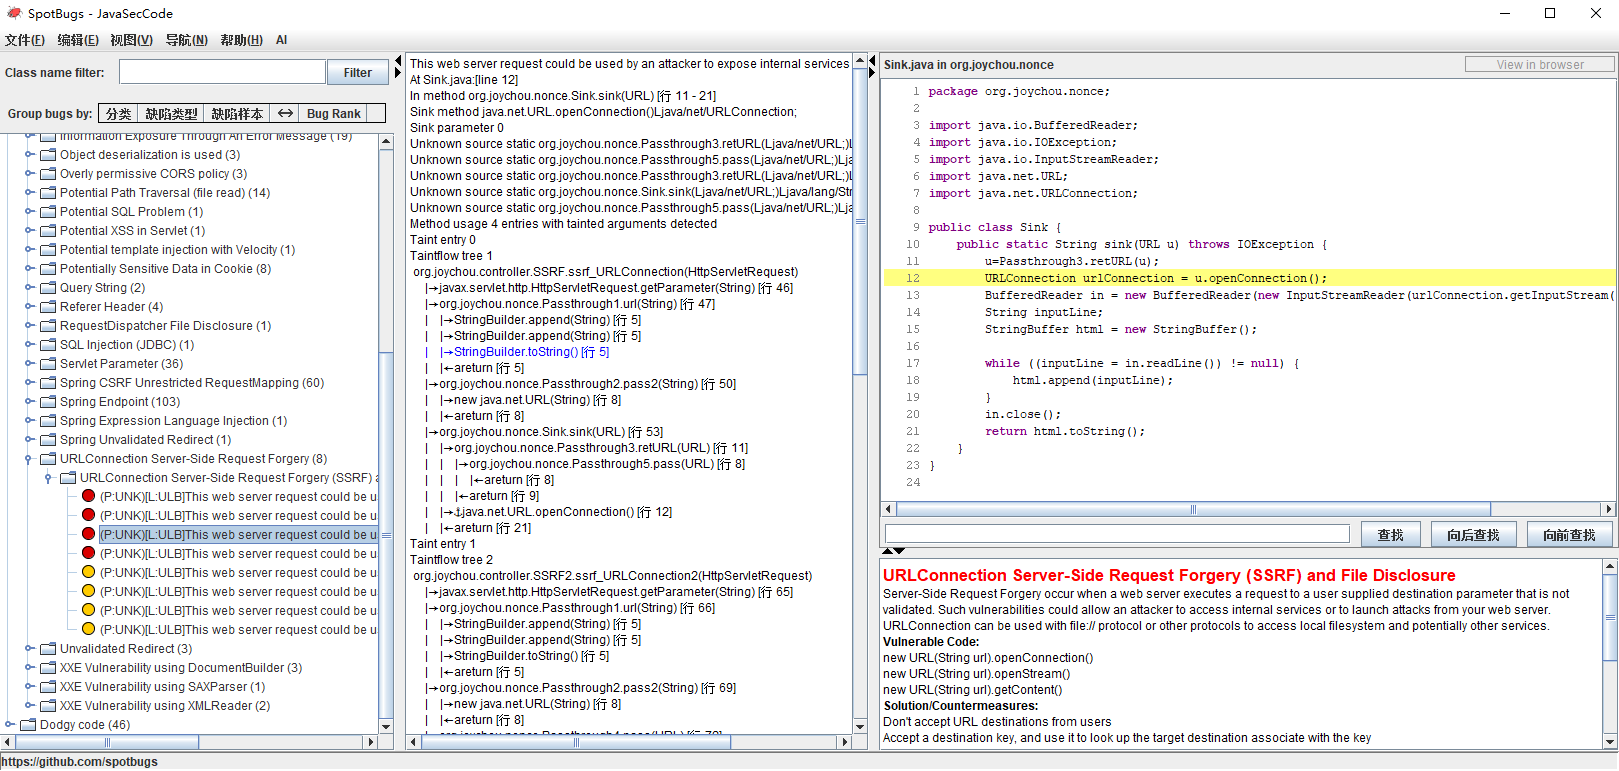
\includegraphics[width=0.8\linewidth]{FIGs/chapter4/taintAnalysis.png}
    \caption{污点分析结果界面}\label{show:taint}
\end{figure} 

图~\ref{show:taint} 展示了系统污点分析结果界面,该界面主要沿用了 Spotbugs 界面,在菜单栏可以新建,读取,保存扫描项目,对 UI 进行调整以及进行预测。左上方窗口显示了按类型整理的漏洞实例,由于用户还未对漏洞进行预测和标记,因此每个叶子节点的开头显示为“[P:UNK][L:ULB]”,左下方显示了一个漏洞实例的污点传播树——这是本系统的主要改进之处,右上方为对应的程序代码,右下方为关于该漏洞的解释信息。

图~\ref{show:settingServer} 展示了设置预测服务器的界面,点击上方菜单栏“AI”中的“Setting Remote Server”将会出现该界面,设置预测服务器是进行误报预测的首要步骤,在设置服务器窗口中,用户需要指定服务器的 URL 地址和管理员发放的 token。

% 设置预测服务器
 \begin{figure}[H]
     \centering
     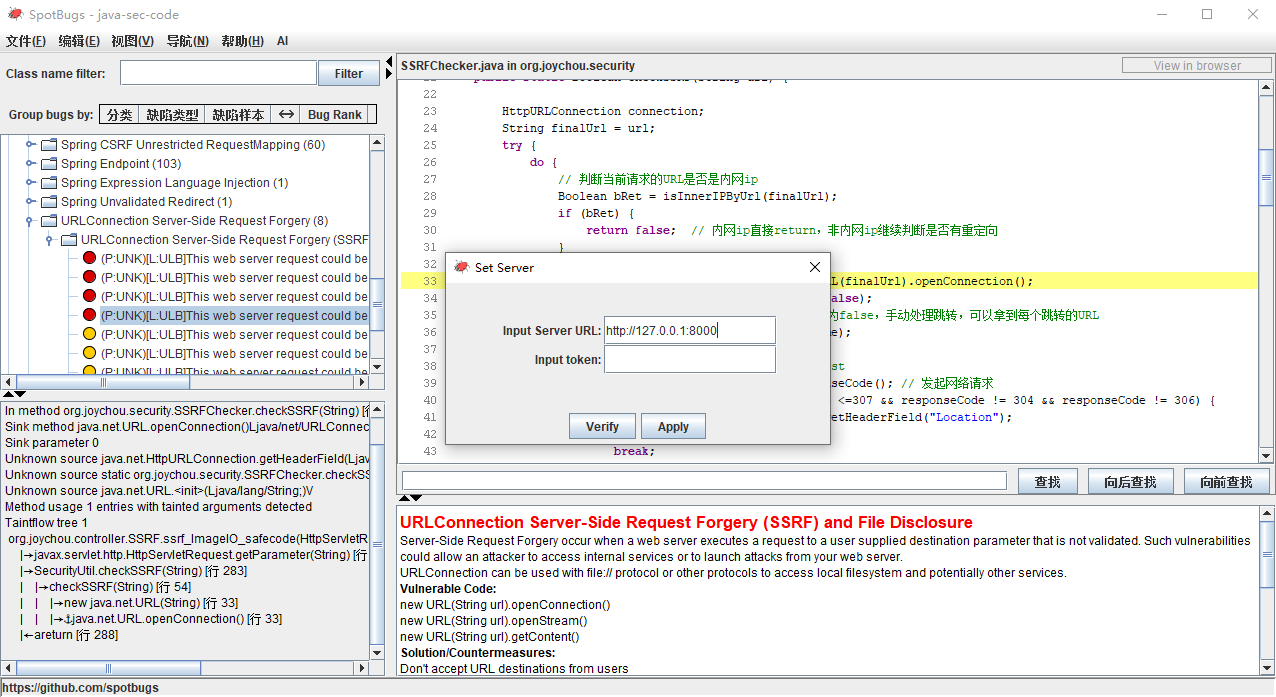
\includegraphics[width=0.8\linewidth]{FIGs/chapter4/settingServer.png}
     \caption{设置预测服务器界面}\label{show:settingServer}
 \end{figure} 

点击上方菜单栏“AI”中的“Slice and Predict”按钮,系统将对污点分析结果进行误报预测,图~\ref{show:predictResult} 展示了预测后一个被预测为误报的漏洞实例,在左上方,可以看到该漏洞实例的叶子节点已经变灰,且预测显示为“[P:FP]”(误报),在左下方,可以看到被预测为清洁函数的污染流已经由有清洁标记标注,这些标记用于向用户解释系统为何将其预测为误报。

% 预测结果
\begin{figure}[H]
    \centering
    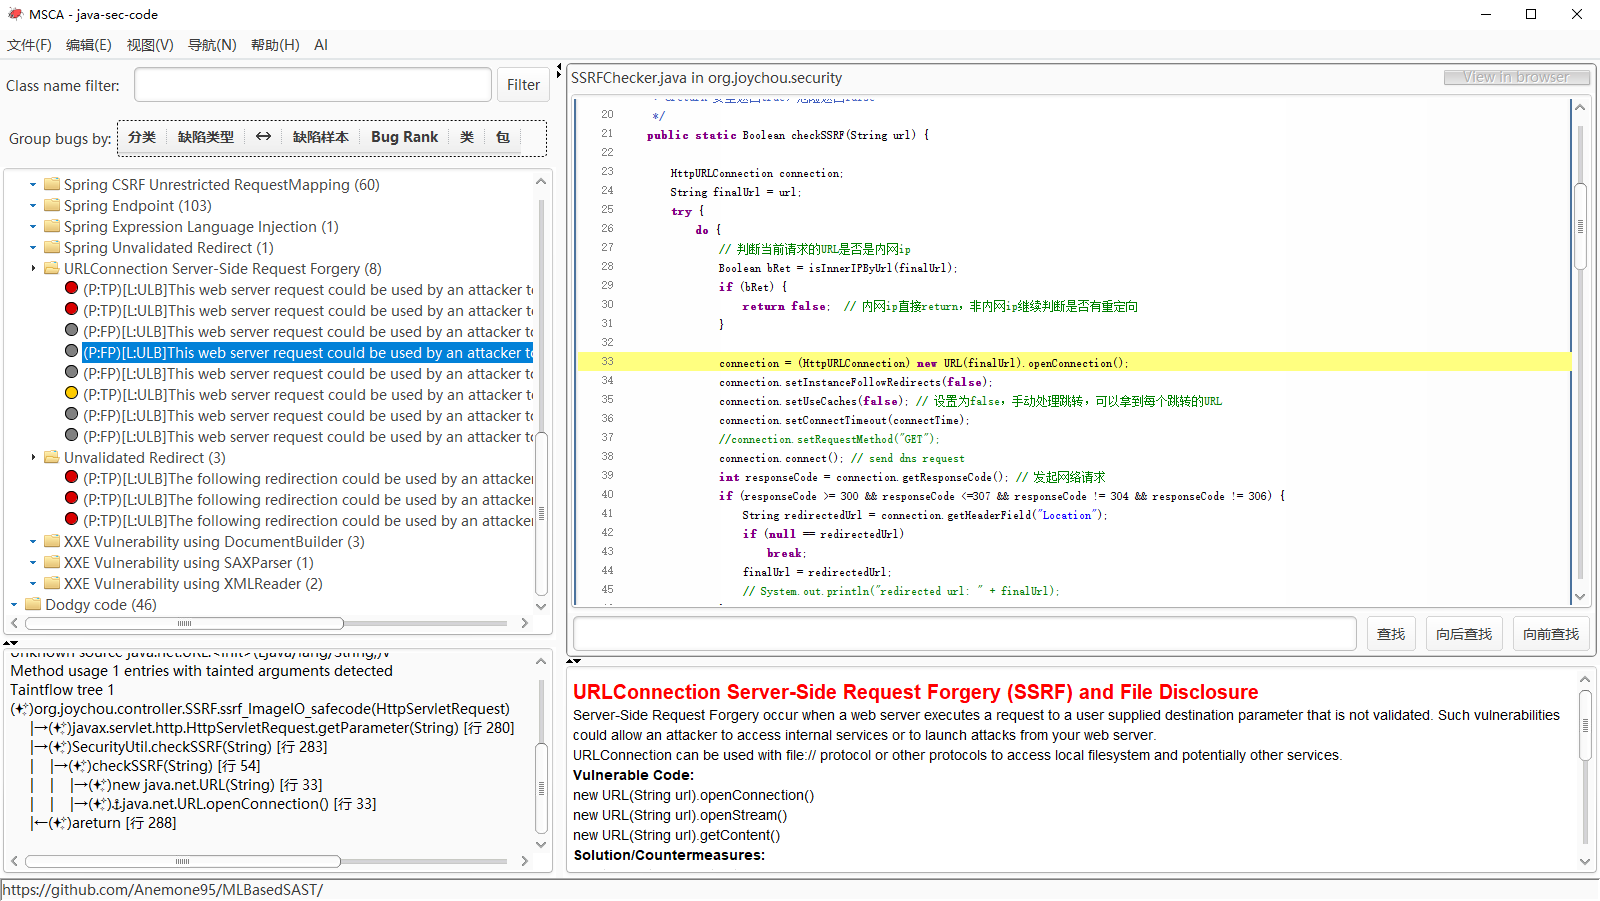
\includegraphics[width=0.8\linewidth]{FIGs/chapter4/predictResult.png}
    \caption{预测结果展示}\label{show:predictResult}
\end{figure}

另外,可以看到图中的代码正是第二章中图~\ref{taintcase2} 中的代码,根据第二章的分析,该代码是为有效的 SSRF 修复代码,而本系统已经能够做出正确的预测,这证明了本系统确实可以根据先前的学习,排除误报。

对于报告中真实存在的漏洞,用户可以对其标记为正报,右击漏洞实例选择“Label as True Positive”即可弹出标记正报的界面,如图~\ref{show:labelTP} 所示,标记正报时用户必须在下拉菜单中选择一棵真实可以利用的污点传播树,点击提交后标记完成,完成后系统会更新左侧漏洞树,将“[L:ULB]”(未标记)转变为“[L:TP]”(标记为正报)。

% 标记正报
\begin{figure}[H]
    \centering
    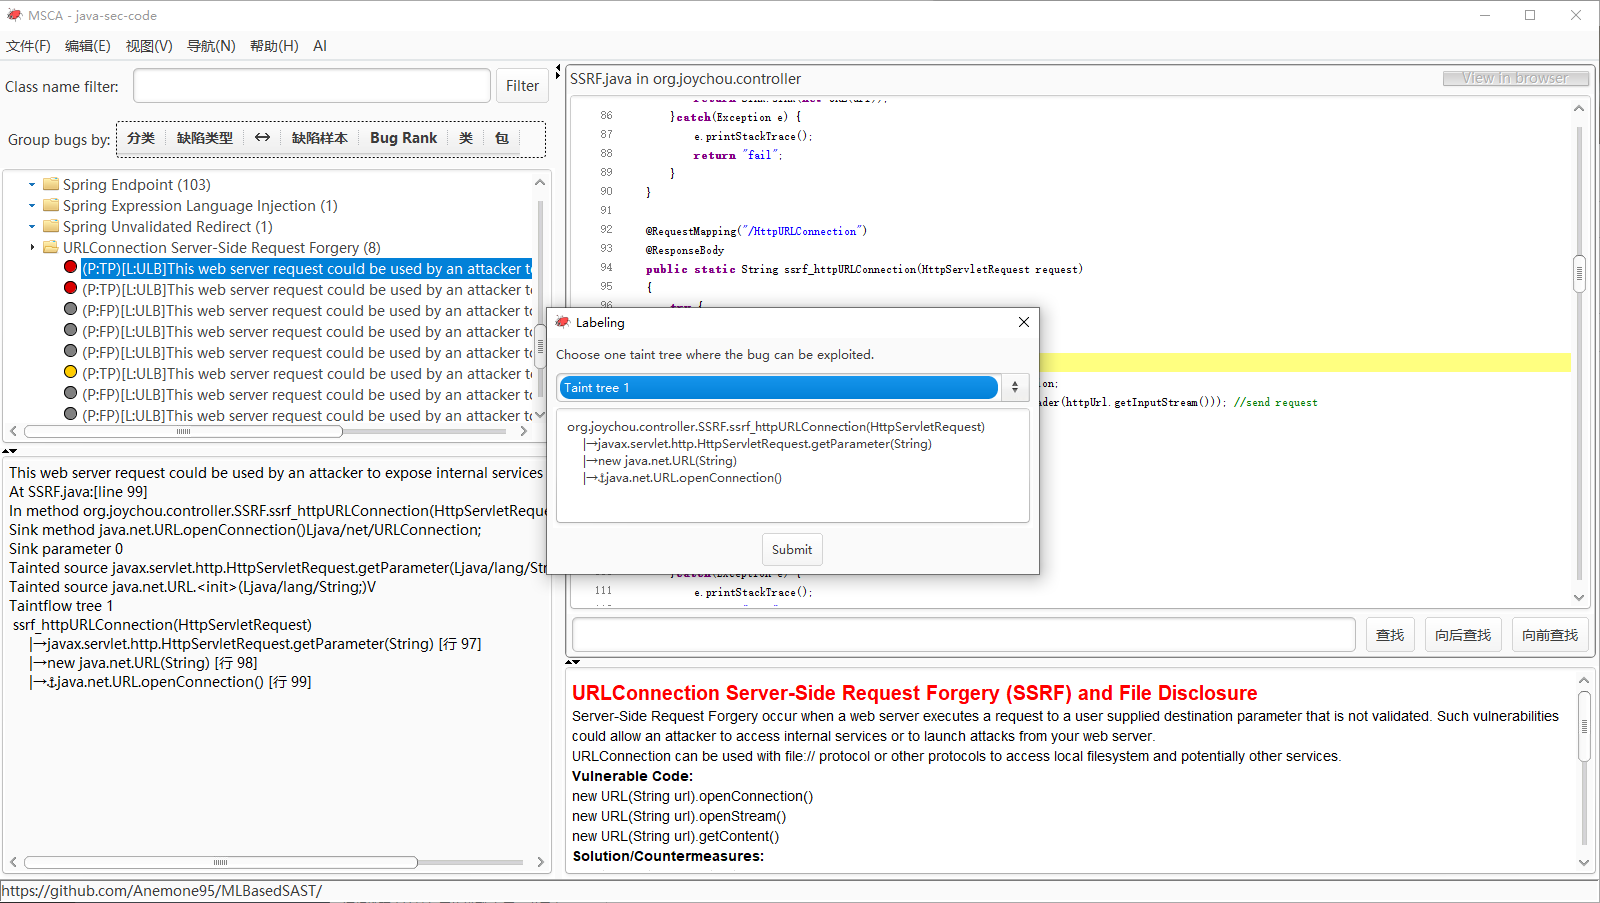
\includegraphics[width=0.8\linewidth]{FIGs/chapter4/labelTP.png}
    \caption{标记正报界面}\label{show:labelTP}
\end{figure}

对于报告中不可利用的正报漏洞,用户可以将其标记为误报,右击漏洞实例选择“Label as False Positive”即可弹出标记误报的界面,如图~\ref{show:labelFP} 所示。

% 标记误报
\begin{figure}[H]
    \centering
    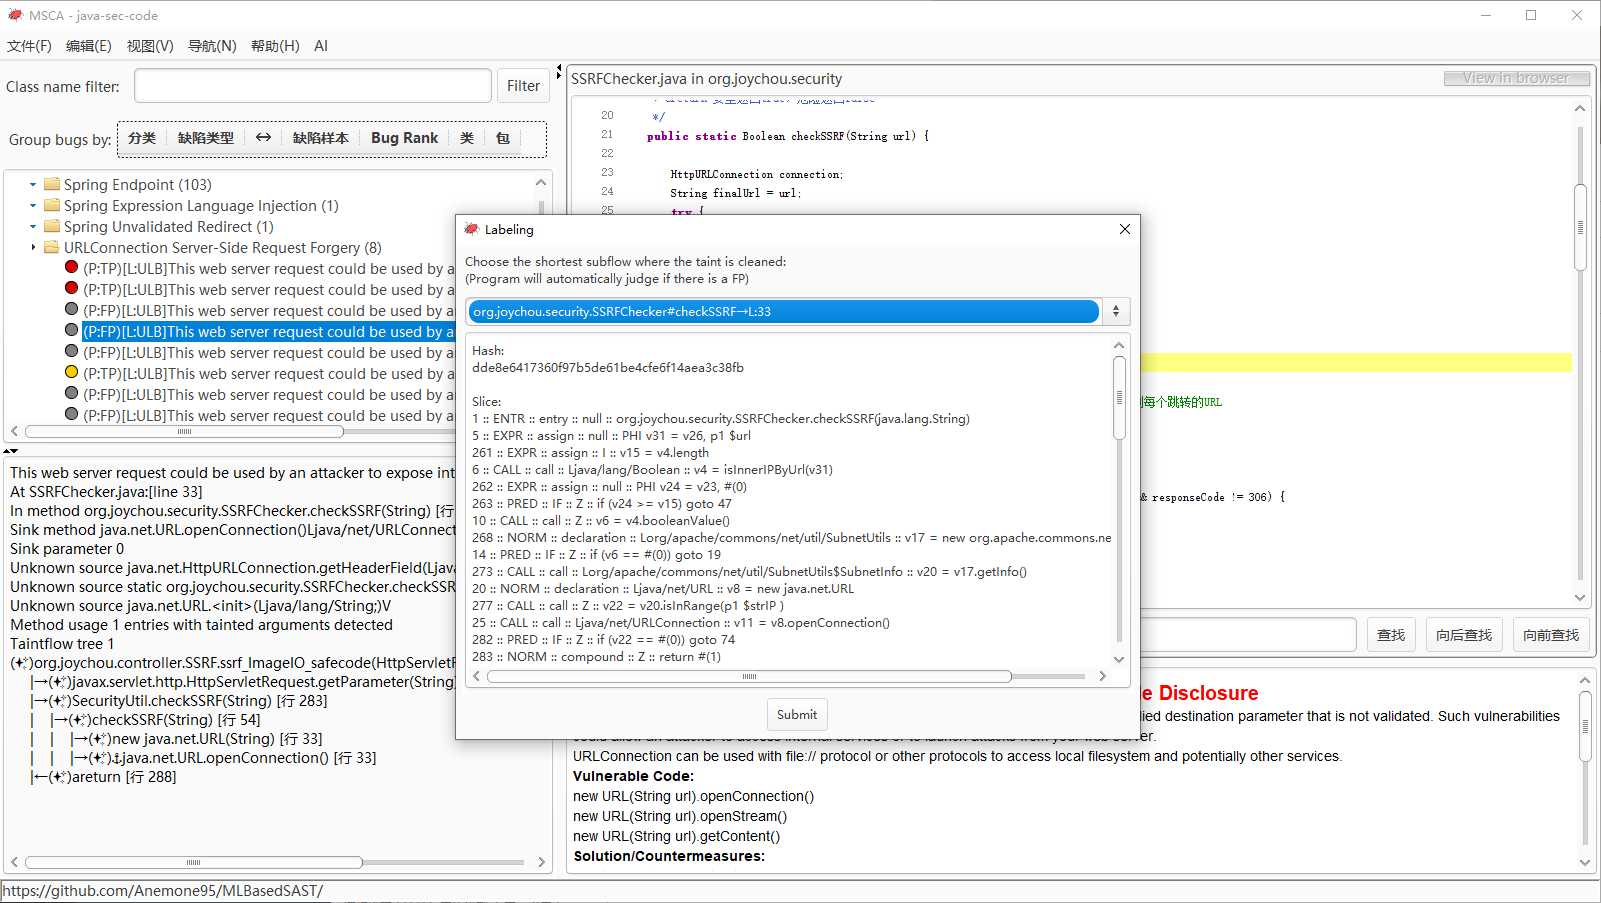
\includegraphics[width=0.8\linewidth]{FIGs/chapter4/labelFP.png}
    \caption{标记误报界面}\label{show:labelFP}
\end{figure}


标记误报时用户需要在下拉菜单中指定一条污染流,同时用户可以在下方看到关于此污染流的切片内容,对误报的标记实际是对安全的污染流标记,标记完成后系统会重新计算并更新漏洞树,用户可以多次点击标记,直至该漏洞的标记变为“[L:FP]”(标记为误报)。




